\documentclass[twoside,11pt]{article}

% JMLR style (https://github.com/JmlrOrg/jmlr-style-file). jmlr2e loads natbib, graphicx, hyperref.
\usepackage{jmlr2e}
\usepackage{booktabs}
\usepackage{array}
\usepackage{lastpage}
\usepackage{xcolor}

% Heading arguments are {volume}{year}{pages}{date submitted}{date published}{paper id}{author-full-names}
\jmlrheading{}{2026}{1-\pageref{LastPage}}{11/26}{}{}{Giuseppe Maulucci, Tommaso Marchetti and Marco De Spirito}
\ShortHeadings{Regularization under data repetition}{Maulucci, Marchetti and De Spirito}
\firstpageno{1}

\newcommand{\wdec}{\mathrm{wd}}
\newcommand{\nats}{nats}
\newcommand{\pending}[1]{\textcolor{red}{[pending: #1]}}

\setlength{\emergencystretch}{2em}
\begin{document}

\title{Regularization under Data Repetition: A Controlled Benchmark of Thirteen Methods for Data-Constrained Language-Model Pretraining}

\author{\name Giuseppe Maulucci \email giuseppe.maulucci@unicatt.it \\
       \addr Universit\`a Cattolica del Sacro Cuore\\
       Rome, Italy
       \AND
       \name Tommaso Marchetti \email [email] \\
       \addr Universit\`a Cattolica del Sacro Cuore\\
       Rome, Italy
       \AND
       \name Marco De Spirito \email [email] \\
       \addr Universit\`a Cattolica del Sacro Cuore\\
       Rome, Italy}

\editor{}

\maketitle

\begin{abstract}%
Pretraining below the data wall repeats the data, and regularization is the usual remedy. Published comparisons test regularizers one at a time against weakly tuned baselines. We compare thirteen regularization methods in one fixed setting: GPT-2-style decoders of 30M and 51M parameters, a pinned 160M-token corpus, 2,432 steps, and two data regimes at identical compute, 10M tokens repeated 16 times or 159M tokens seen once. Every method gets the same tuning budget with the learning rate in the grid, finals share seeds, and the analysis was fixed in advance. In the registered matrix no method beats tuned AdamW, whose decay rate is far above single-pass practice. Constant post-step decays, constrained regularization, no decay and schedule-free AdamW lose 0.13 to 0.41 nats under repetition. Muon gains 0.24 nats single-pass and loses that gain under repetition. A grid extension showed that cautious weight decay, which shrinks only the coordinates whose update already moves toward zero, tolerates three times AdamW's decay. A second pre-registered protocol on held-out seeds confirms its gain at 51M parameters ($-0.065$ nats, $p = 0.0001$). The gain is clear only at sixteen epochs and has the same sign at 125M. Code, protocols and run journals are released.
\end{abstract}

\begin{keywords}
weight decay, data-constrained pretraining, language models, regularization, benchmark
\end{keywords}

\section{Introduction}
\label{sec:intro}

Pretraining corpora of high quality are finite. Models trained beyond the available unique tokens repeat their data for several epochs, and repetition degrades the loss that a given compute budget buys \citep{muennighoff2023scaling}. Regularization is the standard answer. Weight decay, dropout, averaging of the weights, constrained regularization, cautious and stable variants of decay, schedule-free optimization and orthogonalized updates all claim to improve generalization, and most of these claims come from single-method papers.

Three features of those papers make their results hard to compare. First, the learning rate is often fixed while the regularizer is tuned, although the learning rate interacts with every regularizer. Second, the baseline receives a smaller tuning budget than the proposed method. Third, the data regime is not controlled: a method evaluated at one epoch over abundant data may behave differently when the same data are repeated sixteen times.

This paper reports a controlled comparison that removes these three confounders. We fix one architecture, one corpus, one compute budget per run and one tuning protocol, and we run thirteen methods under it. The protocol tunes every method on a grid that always includes the learning rate, extends the grid once when the winner sits on an edge, and retrains the winner on three seeds shared by all methods. Two arms spend the same 2,432 steps and 159.4M tokens: one repeats 10M unique tokens for 16 epochs, the other sees 159M unique tokens once. The analysis was fixed before any run: paired contrasts against AdamW, Holm correction, bootstrap intervals and a paired equivalence test. We confirm the top of the ranking at a larger model size, and we test the one post-registration finding, on cautious weight decay, in a second protocol fixed before its runs.

The paper makes four contributions.
\begin{enumerate}
\item A pre-registered, equal-cost protocol for comparing regularizers under data repetition, with a same-compute single-pass control that turns ``A beats B'' into ``A beats B because of repetition'' or not, and a released pipeline in which a new method enters with one registry entry (Section~\ref{sec:impl}).
\item Paired evidence on thirteen methods at two model sizes, with bootstrap intervals, Holm-adjusted $p$-values and equivalence tests.
\item Three empirical findings. Strong decoupled weight decay is the operating point under repetition, and constant-rate decays do not replace it. Muon's advantage is specific to the single-pass regime and depends on early stopping. An exponential moving average of the weights is the only addition that does not lose, and its gain is within the resolution of the design. Cautious weight decay with a decay three times stronger than AdamW's beats AdamW under sixteen-fold repetition; a pre-registered test on held-out seeds confirms the gain, and a lower effective decay does not explain it.
\item A methodological finding. GPU non-determinism acting on a single tuning seed moved final results by up to 0.12 nats in an independent replicate. Benchmarks at this scale must pair tuning seeds or report the variance of the tuning winner.
\end{enumerate}

\section{Related Work}
\label{sec:related}

\paragraph{Data-constrained pretraining.}
\citet{muennighoff2023scaling} fit scaling laws to repeated data and found that up to four epochs cost little and that the value of repeated tokens then decays. Their experiments use one optimizer configuration. Three recent studies tune the regularization of the repeated-data recipe. \citet{kim2026infinite} find an optimal weight decay 30 times larger than standard practice when epoching over fixed data, and combine it with parameter scaling and ensembling. \citet{lovelace2026prescriptive} add an overfitting penalty to the Chinchilla law and report that a weight decay of 1.0 cuts the fitted overfitting coefficient by about 70\%. \citet{xu2026dataconstrained} add a masked-input auxiliary loss on top of strong weight decay and propose a scaling law that couples model size and data size. These studies tune weight decay inside one recipe or add one regularizer to it. None compares the families of regularizers with each other under one protocol, and none controls the data regime at identical compute. We hold compute fixed and ask which regularizer makes repetition cheaper.

\paragraph{Weight decay and its variants.}
AdamW decouples the decay from the gradient step and ties its per-step rate to the learning-rate schedule \citep{loshchilov2019decoupled}. Later work studies why decay helps modern networks at all \citep{dangelo2024why}. Scheduled weight decay (AdamS) scales the decay rate with the gradient norm \citep{xie2023overlooked}. Cautious weight decay applies the decay only to coordinates whose decay direction agrees with the update \citep{chen2026cautious}. Constrained parameter regularization replaces the penalty with a constraint on a norm statistic and adapts its Lagrange multiplier \citep{franke2024cpr}. Post-step constant decays shrink the weights by a fixed fraction after each step, independently of the learning-rate schedule; the Fair and Huber profiles saturate the shrinkage for large weights \citep{fair1974robust,huber1964robust}. We include three such decays as entrants.

\paragraph{Averaging, dropout and schedule-free optimization.}
An exponential moving average of the weights at evaluation time reduces the loss of Adam-trained language models \citep{moralesbrotons2024ema}. Dropout \citep{srivastava2014dropout} is the classical regularizer for repeated data and is usually turned off in large-scale pretraining. Schedule-free AdamW replaces the learning-rate schedule by an interpolation between an averaged and a fast iterate \citep{defazio2024road}.

\paragraph{Orthogonalized updates.}
Muon orthogonalizes the momentum of two-dimensional weights with a Newton--Schulz iteration \citep{jordan2024muon} and scales to large pretraining runs with decoupled decay \citep{liu2025muon}. Its reported gains come from single-pass training. We measure it under repetition as well.

\paragraph{Benchmarks of optimizers and regularizers.}
Optimizer benchmarks show that tuning budget and baseline strength decide most reported gains \citep{schmidt2021descending,dahl2023benchmarking}. Recent comparisons of pretraining optimizers reach the same conclusion at larger scale \citep{wen2026fantastic,semenov2025benchmarking}. None of them controls the data regime. Our protocol adopts their lesson on tuning and adds the regime control.

\section{Benchmark Design}
\label{sec:design}

\subsection{Setting}

\paragraph{Data.}
We use FineWeb-Edu \texttt{sample-10BT} \citep{penedo2024fineweb} at a pinned revision, tokenized with the GPT-2 byte-pair encoder, with document-level splits. The training file holds 160,000,000 tokens; the validation and test files hold 3.32M and 3.30M tokens. We record the SHA-256 of every split and check it on every machine before a run. A run with $D$ unique tokens reads the first $D$ tokens of the training file.

\paragraph{Model.}
The model is a pre-LayerNorm GPT with learned positions, tied embeddings and a context of 1,024 tokens. Size XS has 6 layers, width 384, 6 heads and 30,357,504 parameters. Size S has 8 layers, width 512, 8 heads and 51,500,032 parameters.

\paragraph{Optimization.}
Every run takes 2,432 optimizer steps with 64 sequences of 1,024 tokens per step (65,536 tokens per step, 159,383,552 tokens per run). The Adam family \citep{kingma2015adam} uses betas $(0.9, 0.95)$ and epsilon $10^{-8}$. Gradients are clipped at norm 1.0. Training uses bf16 autocast and \texttt{torch.compile}. The learning rate warms up linearly over 2\% of the steps (48) and decays linearly to zero, except for schedule-free AdamW, which uses its own warm-up and no decay. Dropout is zero unless it is the tuned hyperparameter. Decay applies to two-dimensional weights (linear layers, token and position embeddings) and never to biases or LayerNorm parameters; this scope is the same for every method.

\paragraph{Two arms at identical compute.}
Arm R16 trains on $D = 10{,}000{,}000$ unique tokens for 16 epochs (152 steps per epoch), with a fresh seeded order each epoch. Arm R1 trains on $D = 159{,}383{,}553$ unique tokens for one epoch. The two arms differ only in how many distinct tokens the 2,432 steps see.

\paragraph{Evaluation.}
Validation loss is measured every 76 steps on the first $2^{20}$ validation tokens (32 evaluations per run). The checkpoint with the lowest validation loss is restored through a verified restore routine and evaluated on the full test split. The end-of-training model is evaluated as well. No run stops early.

\subsection{Methods}

Table~\ref{tab:methods} lists the thirteen methods, their mechanism and their tuning grids. The two values of each second axis bracket the same peak per-step shrinkage, about $10^{-4}$ and $5\times10^{-4}$, in each method's native units. AdamW+dropout and AdamW+EMA inherit AdamW's tuned weight decay and spend their configurations on their own hyperparameter. We use the reference implementations of AdamS \citep{xie2023overlooked}, CPR \citep{franke2024cpr}, schedule-free AdamW \citep{defazio2024road} and Muon \citep{jordan2024muon}.

\begin{table}[t]
\centering
\footnotesize
\setlength{\tabcolsep}{3.5pt}
\begin{tabular}{@{}l p{3.9cm} l l p{2.6cm}@{}}
\toprule
Method & Mechanism & Learning rates & Second axis & Fixed \\
\midrule
Baseline & no decay & 5e-4, 1.5e-3, 4.5e-3 & -- & \\
AdamW & decoupled decay $\mathrm{lr}_t \cdot \wdec$ & same & wd 0.1, 0.5 & \\
AdamW+dropout & AdamW with dropout & same & dropout 0.1, 0.3 & wd of AdamW's winner \\
AdamW+EMA & AdamW, EMA of the weights at evaluation & same & ema 0.99, 0.999 & wd of AdamW's winner \\
CWD & cautious weight decay & same & wd 0.1, 0.5 & \\
AdamS & scheduled weight decay & same & wd 1e-4, 1e-3 & \\
CPR & constrained parameter regularization & same & warm start 0, 250 & \\
SF-AdamW & schedule-free AdamW & same & wd 0.1, 0.5 & warm-up 48 steps \\
Muon & Muon on hidden matrices, Adam elsewhere & 7e-3, 2e-2, 6e-2 & wd 0.005, 0.02 & aux lr 1.5e-3, aux wd 0.1 \\
Muon+Const & Muon, post-step constant decay & 7e-3, 2e-2, 6e-2 & $\rho$ 1e-4, 5e-4 & aux lr 1.5e-3 \\
Const & $w \leftarrow w - \rho w$ & 5e-4, 1.5e-3, 4.5e-3 & $\rho$ 1e-4, 5e-4 & \\
Const-Fair & $w \leftarrow w - \rho w / (1 + |w|/\delta)$ & same & $\rho$ 1e-4, 5e-4 & $\delta = 0.1$ \\
Const-Huber & $w \leftarrow w - \rho\,\mathrm{clamp}(w, \pm\delta)$ & same & $\rho$ 1e-4, 5e-4 & $\delta = 0.1$ \\
\bottomrule
\end{tabular}
\caption{The thirteen methods and their tuning grids. ``Same'' means the Adam learning-rate grid. The warm start of CPR is 0 (inflection point) or 250 steps.}
\label{tab:methods}
\end{table}

\subsection{Tuning Protocol}

Figure~\ref{fig:protocol} summarizes the design. Each method is tuned on one seed (42) over three learning rates and two values of its second axis, six configurations in all. The configuration with the lowest best-checkpoint validation loss wins. If the winner sits at an end of an axis, that axis is extended by one step outward (learning rate $\times 3$ or $\div 3$; weight decay and $\rho$ $\times 5$ or $\div 5$; the AdamS decay $\times 10$ or $\div 10$; ema $0.999 \to 0.9999$ or $0.99 \to 0.9$; dropout $0.3 \to 0.5$ or $0.1 \to 0.03$; the CPR warm start $250 \to 1000$), at most once per axis. The winner is then retrained on seeds 1001, 1002 and 1003, the same seeds for every method, so that all comparisons are paired. In arm R1 each method runs at its R16-winning configuration and at one weaker-regularization variant of it (AdamW+dropout only at its R16 configuration), with two final seeds. The S phase repeats the R16 search at 51.5M parameters for AdamW and for the four methods with the lowest mean test loss at XS; the selection rule was fixed in advance and applied mechanically.

\begin{figure}[t]
\centering
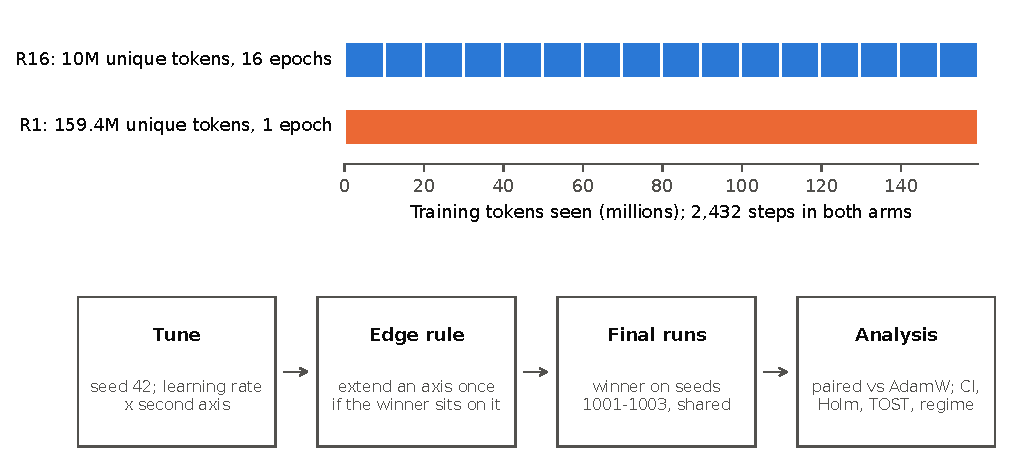
\includegraphics[width=\textwidth]{figures/F1_protocol.pdf}
\caption{The design. Top: the two arms spend the same 2,432 steps and 159.4M training tokens; R16 repeats 10M unique tokens sixteen times, R1 sees 159.4M unique tokens once. Bottom: the pipeline applied to every method in each arm.}
\label{fig:protocol}
\end{figure}

\subsection{Pre-registered Analysis}

The primary outcome is the test loss at the best-validation checkpoint in arm R16 at size XS. Every method is contrasted with AdamW by a paired $t$-test over the shared seeds, with Holm's step-down correction within the table. We report a percentile bootstrap interval of the paired difference (10,000 resamples) and a paired two one-sided test of equivalence with a margin of 0.01 nats. A contrast is called ``worse'' or ``better'' when it survives Holm, ``parity'' when the equivalence test passes, and ``inconclusive'' otherwise. Secondary outcomes are the end-of-training test loss, the same contrasts in arm R1, the regime effect, defined as the difference between a method's contrast with AdamW in R16 and in R1 with a bootstrap interval that resamples the seeds of each arm independently, and the confirmation at size S. The protocol, the grids, the edge rule and the analysis script were committed before the first run.

\subsection{Implementation}
\label{sec:impl}

One training routine serves every method. A run journal records every grid point and every final run under the full configuration; a re-invocation replays journaled points, so an extended grid never repeats a run and the finals follow the winner. The best-checkpoint restore verifies a parameter fingerprint and re-evaluates the restored model. The code, the journals and the result files are released with the paper.

\paragraph{Adding a method.}
A new method enters the benchmark with one entry in the method registry, which names its optimizer constructor and its second tuning axis, and one command per arm. The driver tunes it on the shared learning-rate grid, applies the edge rule, retrains the winner on the shared seeds and writes a result file in the format the analysis reads. Runs added after registration carry a tag and appear in the sensitivity section, never in the registered tables. The cost per arm is 6 to 12 tuning runs and the final runs: about three GPU-hours at XS and four at S on an RTX 3090.

\section{Results}
\label{sec:results}

\subsection{Primary Outcome: XS, Repeated Data}

Table~\ref{tab:xs_r16} and Figure~\ref{fig:contrasts} report the primary outcome. AdamW reaches a mean test loss of 4.487 (sd 0.042) with learning rate $4.5\times10^{-3}$ and weight decay 2.5, the latter reached through the one allowed extension. No contrast survives the Holm correction at $n = 3$. The bootstrap intervals separate two groups. AdamW+EMA ($-0.024$, CI95 $[-0.084, +0.020]$), Muon ($-0.021$, $[-0.067, +0.002]$), AdamS, Muon+Const, AdamW+dropout and CWD lie within 0.05 nats of AdamW with intervals that include zero. Const-Huber ($+0.132$), Const ($+0.171$), CPR ($+0.234$), Const-Fair ($+0.267$), Baseline ($+0.327$) and SF-AdamW ($+0.412$) lie above AdamW with intervals that exclude zero.

\begin{table}[t]
\centering
\footnotesize
\resizebox{\textwidth}{!}{%
\begin{tabular}{@{}lrrrcrrl@{}}
\toprule
Method & mean & sd & diff & bootstrap CI95 & $p$ & $p$ (Holm) & winner \\
\midrule
AdamW+EMA & 4.4637 & 0.0202 & $-0.0235$ & $[-0.0842, +0.0199]$ & 0.531 & 1.000 & lr 4.5e-3, ema 0.99, wd 2.5 \\
Muon & 4.4661 & 0.0051 & $-0.0212$ & $[-0.0670, +0.0024]$ & 0.454 & 1.000 & lr 0.06, wd 0.1 \\
\textbf{AdamW} & 4.4872 & 0.0420 & & & & & lr 4.5e-3, wd 2.5 \\
AdamS & 4.4914 & 0.0345 & $+0.0042$ & $[-0.0601, +0.0720]$ & 0.923 & 1.000 & lr 1.35e-2, wd 1e-4 \\
Muon+Const & 4.4978 & 0.0057 & $+0.0105$ & $[-0.0429, +0.0450]$ & 0.735 & 1.000 & lr 0.06, $\rho$ 2.5e-3 \\
AdamW+dropout & 4.5005 & 0.0267 & $+0.0133$ & $[-0.0315, +0.0582]$ & 0.659 & 1.000 & lr 4.5e-3, dropout 0.03, wd 2.5 \\
CWD & 4.5283 & 0.0089 & $+0.0411$ & $[-0.0087, +0.0707]$ & 0.242 & 1.000 & lr 4.5e-3, wd 2.5 \\
Const-Huber & 4.6192 & 0.0411 & $+0.1320$ & $[+0.0672, +0.2070]$ & 0.083 & 0.584 & lr 4.5e-3, $\rho$ 2.5e-3 \\
Const & 4.6582 & 0.0290 & $+0.1709$ & $[+0.1269, +0.2258]$ & 0.028 & 0.222 & lr 4.5e-3, $\rho$ 2.5e-3 \\
CPR & 4.7214 & 0.0074 & $+0.2341$ & $[+0.1774, +0.2653]$ & 0.014 & 0.133 & lr 1.5e-3, warm start 250 \\
Const-Fair & 4.7539 & 0.0810 & $+0.2667$ & $[+0.2057, +0.3069]$ & 0.013 & 0.133 & lr 4.5e-3, $\rho$ 2.5e-3 \\
Baseline & 4.8140 & 0.0161 & $+0.3267$ & $[+0.2625, +0.3711]$ & 0.010 & 0.110 & lr 1.5e-3 \\
SF-AdamW & 4.8992 & 0.0227 & $+0.4120$ & $[+0.3487, +0.4663]$ & 0.007 & 0.082 & lr 4.5e-3, wd 2.5 \\
\bottomrule
\end{tabular}}
\caption{XS, R16 (10M tokens $\times$ 16 epochs): test loss at the best-validation checkpoint, $n = 3$ seeds. ``diff'' is the paired difference from AdamW; $p$ from the paired $t$-test; Holm within the table.}
\label{tab:xs_r16}
\end{table}

\begin{figure}[t]
\centering
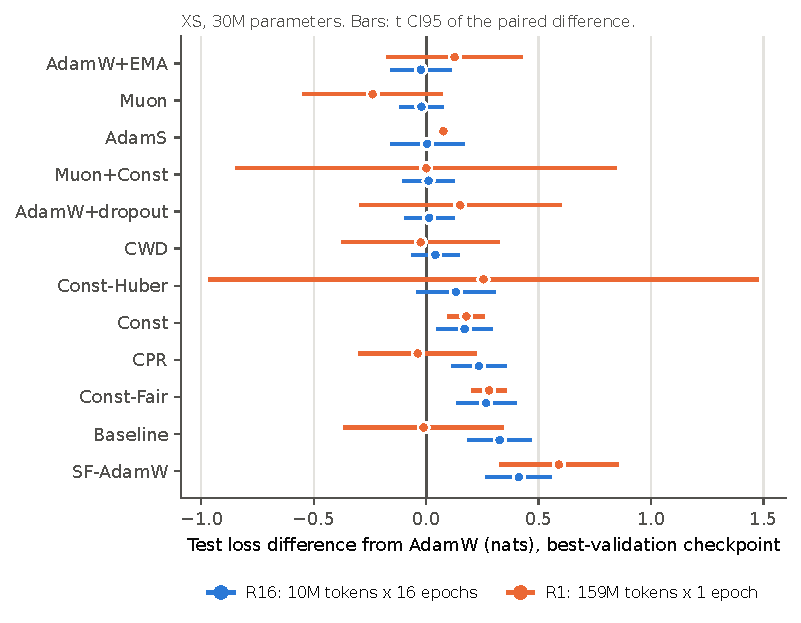
\includegraphics[width=0.8\textwidth]{figures/F2_contrasts_r16_r1.pdf}
\caption{Paired difference from AdamW in test loss at the best-validation checkpoint, XS, in the repeated-data arm (R16, $n = 3$) and in the single-pass arm (R1, $n = 2$). Bars: bootstrap CI95.}
\label{fig:contrasts}
\end{figure}

Most winners sit on a grid edge after the one allowed extension: AdamW, CWD and SF-AdamW on the weight-decay edge (2.5), the three constant decays on the $\rho$ edge ($2.5\times10^{-3}$), Muon on its weight-decay edge and AdamS on the learning-rate edge. Section~\ref{sec:edges} returns to this point.

\subsection{Control Arm and Regime Effect}
\label{sec:r1}

In arm R1 (Table~\ref{tab:xs_r1} and Figure~\ref{fig:contrasts}) the ranking changes. Muon leads by $-0.238$ nats (CI95 $[-0.263, -0.214]$). CPR ($-0.037$), CWD ($-0.024$) and Baseline ($-0.012$) sit at or below AdamW: with a single pass over 159M tokens, weight decay buys nothing. AdamS ($+0.077$), AdamW+EMA ($+0.126$), AdamW+dropout ($+0.151$), the constant decays ($+0.18$ to $+0.28$) and SF-AdamW ($+0.590$) lose to AdamW.

\begin{table}[t]
\centering
\footnotesize
\begin{tabular}{@{}lrrcl@{}}
\toprule
Method & mean & diff & bootstrap CI95 & winner \\
\midrule
Muon & 3.9148 & $-0.2381$ & $[-0.2625, -0.2136]$ & lr 0.06, wd 0.1 \\
CPR & 4.1155 & $-0.0374$ & $[-0.0581, -0.0167]$ & lr 1.5e-3, warm start 250 \\
CWD & 4.1285 & $-0.0243$ & $[-0.0519, +0.0032]$ & lr 4.5e-3, wd 2.5 \\
Baseline & 4.1414 & $-0.0115$ & $[-0.0394, +0.0165]$ & lr 1.5e-3 \\
\textbf{AdamW} & 4.1529 & & & lr 4.5e-3, wd 0.5 \\
Muon+Const & 4.1535 & $+0.0006$ & $[-0.0660, +0.0673]$ & lr 0.06, $\rho$ 5e-4 \\
AdamS & 4.2294 & $+0.0765$ & $[+0.0743, +0.0787]$ & lr 1.35e-2, wd 1e-4 \\
AdamW+EMA & 4.2793 & $+0.1264$ & $[+0.1027, +0.1501]$ & lr 4.5e-3, ema 0.9, wd 2.5 \\
AdamW+dropout & 4.3043 & $+0.1514$ & $[+0.1161, +0.1868]$ & lr 4.5e-3, dropout 0.03, wd 2.5 \\
Const & 4.3316 & $+0.1787$ & $[+0.1723, +0.1852]$ & lr 4.5e-3, $\rho$ 5e-4 \\
Const-Huber & 4.4076 & $+0.2547$ & $[+0.1586, +0.3509]$ & lr 4.5e-3, $\rho$ 5e-4 \\
Const-Fair & 4.4328 & $+0.2799$ & $[+0.2738, +0.2860]$ & lr 4.5e-3, $\rho$ 5e-4 \\
SF-AdamW & 4.7430 & $+0.5901$ & $[+0.5692, +0.6110]$ & lr 4.5e-3, wd 2.5 \\
\bottomrule
\end{tabular}
\caption{XS, R1 (159.4M tokens $\times$ 1 epoch): test loss at the best-validation checkpoint, $n = 2$ seeds.}
\label{tab:xs_r1}
\end{table}

The regime effect (Table~\ref{tab:regime} and Figure~\ref{fig:regime}) is the R16 contrast minus the R1 contrast. A positive value means that the method loses ground to AdamW when the data are repeated. Baseline ($+0.338$, CI95 $[+0.274, +0.402]$), CPR ($+0.272$) and Muon ($+0.217$) lose the most; CWD loses $+0.065$. AdamW+EMA ($-0.150$), AdamW+dropout ($-0.138$), SF-AdamW ($-0.178$) and AdamS ($-0.072$) gain ground under repetition. Const and Const-Fair show no regime effect ($-0.008$ and $-0.013$): they lose to AdamW by the same margin in both regimes. Const-Huber gains some ground under repetition ($-0.123$), but its interval, $[-0.266, +0.020]$, includes zero.

\begin{table}[t]
\centering
\footnotesize
\begin{tabular}{@{}lrrrc@{}}
\toprule
Method & diff R16 & diff R1 & regime effect & CI95 \\
\midrule
SF-AdamW & $+0.4120$ & $+0.5901$ & $-0.1781$ & $[-0.2414, -0.1181]$ \\
AdamW+EMA & $-0.0235$ & $+0.1264$ & $-0.1499$ & $[-0.2106, -0.0915]$ \\
AdamW+dropout & $+0.0133$ & $+0.1514$ & $-0.1381$ & $[-0.2034, -0.0729]$ \\
Const-Huber & $+0.1320$ & $+0.2547$ & $-0.1228$ & $[-0.2655, +0.0200]$ \\
AdamS & $+0.0042$ & $+0.0765$ & $-0.0723$ & $[-0.1366, -0.0045]$ \\
Const-Fair & $+0.2667$ & $+0.2799$ & $-0.0133$ & $[-0.0742, +0.0270]$ \\
Const & $+0.1709$ & $+0.1787$ & $-0.0078$ & $[-0.0519, +0.0471]$ \\
Muon+Const & $+0.0105$ & $+0.0006$ & $+0.0099$ & $[-0.0861, +0.1058]$ \\
CWD & $+0.0411$ & $-0.0243$ & $+0.0654$ & $[+0.0114, +0.1195]$ \\
Muon & $-0.0212$ & $-0.2381$ & $+0.2169$ & $[+0.1693, +0.2645]$ \\
CPR & $+0.2341$ & $-0.0374$ & $+0.2715$ & $[+0.2148, +0.3215]$ \\
Baseline & $+0.3267$ & $-0.0115$ & $+0.3382$ & $[+0.2741, +0.4023]$ \\
\bottomrule
\end{tabular}
\caption{Regime effect: (method $-$ AdamW in R16) $-$ (method $-$ AdamW in R1), XS. CI95 from a bootstrap that resamples the seeds of each arm independently.}
\label{tab:regime}
\end{table}

\begin{figure}[t]
\centering
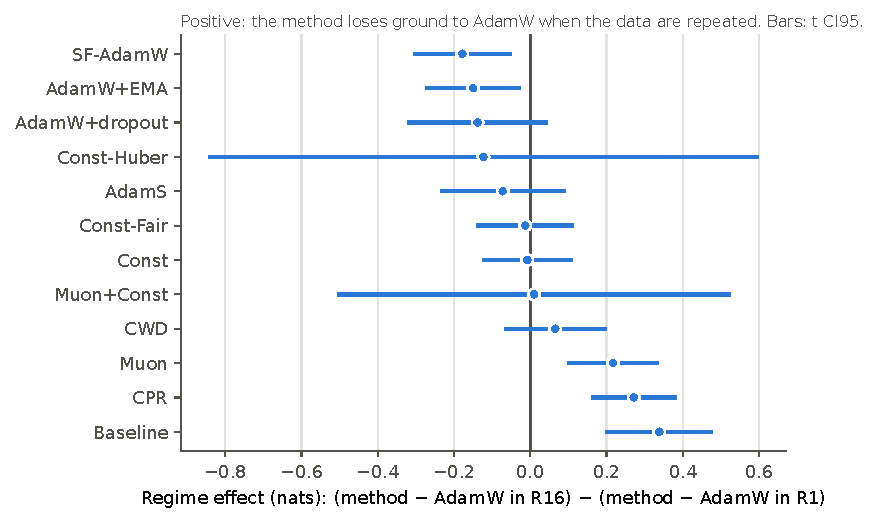
\includegraphics[width=0.8\textwidth]{figures/F3_regime_effect.pdf}
\caption{Regime effect per method, XS. Positive values: the method loses ground to AdamW when the data are repeated. Bars: bootstrap CI95.}
\label{fig:regime}
\end{figure}

\subsection{Confirmation at 51.5M Parameters}

The S phase ran AdamW, AdamW+EMA, Muon, AdamS and Muon+Const in arm R16 (Table~\ref{tab:s} and Figure~\ref{fig:s}). AdamW reaches 4.385 (sd 0.006) with the same winner as at XS. AdamW+EMA improves on it by $-0.024$ nats (CI95 $[-0.033, -0.011]$, $p = 0.069$, Holm 0.21), the same difference as at XS. Muon+Const matches AdamW ($+0.006$, $[+0.000, +0.012]$). Muon loses $+0.051$ ($[+0.046, +0.055]$, Holm 0.010), the only best-checkpoint contrast in the registered tables that survives the correction, with the pre-registered verdict ``worse''. AdamS loses $+0.069$ ($[+0.043, +0.109]$).

\begin{table}[t]
\centering
\footnotesize
\resizebox{\textwidth}{!}{%
\begin{tabular}{@{}lrrrcrrrr@{}}
\toprule
Method & mean & sd & diff & bootstrap CI95 & $p$ & $p$ (Holm) & best epoch & final-ckpt loss \\
\midrule
AdamW+EMA & 4.3615 & 0.0112 & $-0.0236$ & $[-0.0327, -0.0109]$ & 0.069 & 0.208 & 16.0 & 4.36 \\
\textbf{AdamW} & 4.3851 & 0.0059 & & & & & 16.0 & 4.39 \\
Muon+Const & 4.3911 & 0.0034 & $+0.0060$ & $[+0.0000, +0.0122]$ & 0.231 & 0.231 & 10.3 & 5.13 \\
Muon & 4.4356 & 0.0026 & $+0.0505$ & $[+0.0460, +0.0546]$ & 0.002 & 0.010 & 9.7 & 4.89 \\
AdamS & 4.4540 & 0.0413 & $+0.0689$ & $[+0.0433, +0.1094]$ & 0.078 & 0.208 & 16.0 & 4.45 \\
\bottomrule
\end{tabular}}
\caption{S (51.5M parameters), R16: test loss at the best-validation checkpoint, $n = 3$ seeds, with the mean epoch of the best checkpoint and the test loss of the final checkpoint.}
\label{tab:s}
\end{table}

\begin{figure}[t]
\centering
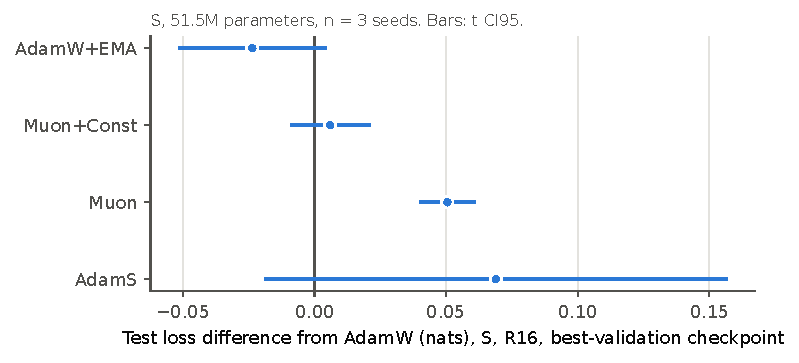
\includegraphics[width=0.75\textwidth]{figures/F5_s_contrasts.pdf}
\caption{Paired difference from AdamW at S, R16, $n = 3$ seeds. Bars: bootstrap CI95.}
\label{fig:s}
\end{figure}

\subsection{Best Checkpoint Against Final Checkpoint}

The primary outcome credits each method with its best-validation checkpoint. The end-of-training checkpoint tells which methods depend on early stopping (Figure~\ref{fig:curves}). At XS in arm R16, AdamW, AdamW+EMA, AdamS, AdamW+dropout and SF-AdamW reach their best validation loss in the last epoch (AdamW+EMA half an epoch earlier on one seed), so the two checkpoints coincide or differ by less than 0.001 nats. Muon peaks at epoch 11.7 and ends 0.15 nats above its best; Muon+Const peaks at epoch 9.7 and ends 0.78 nats above its best; Baseline peaks at epoch 9 and ends 0.22 nats above; CPR peaks at epoch 10.7 and ends 0.12 nats above. At S the pattern is sharper: Muon and Muon+Const peak around epoch 10 and end 0.46 and 0.74 nats above their best checkpoints, while AdamW, AdamW+EMA and AdamS keep improving until the last step. Under repetition, the methods that rely on orthogonalized updates or on no decay memorize the corpus after about ten epochs; strong decoupled decay does not.

\begin{figure}[t]
\centering
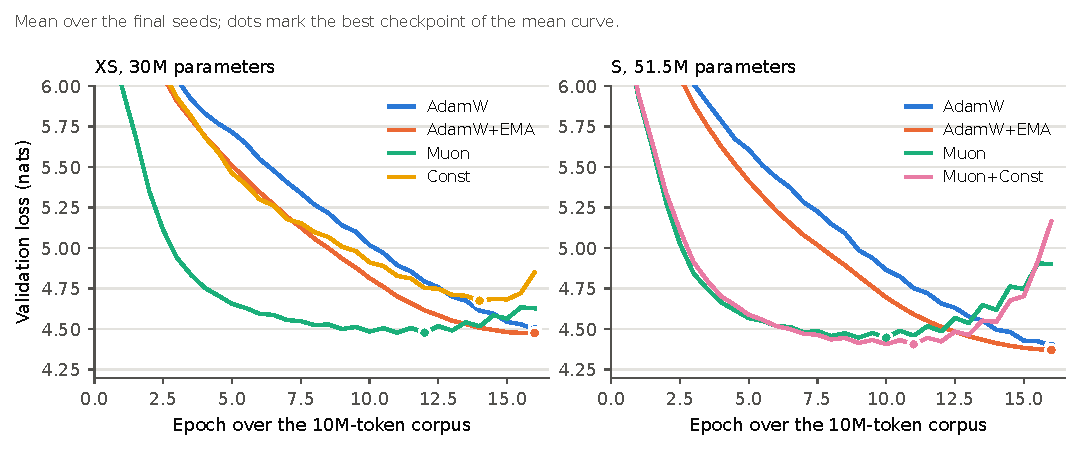
\includegraphics[width=\textwidth]{figures/F4_curves_r16.pdf}
\caption{Validation loss during training in arm R16, mean over the final seeds, at XS (left) and S (right). Dots mark the best checkpoint of the mean curve.}
\label{fig:curves}
\end{figure}

\subsection{Cost}

Throughput at XS ranges from 166,000 to 171,000 tokens per second across methods on the same GPU. The Muon family costs 1.7 to 2.2\% more time than AdamW, CWD 1.0\%, every other method less than 1\%. At S the overheads are 2.3 to 2.4\% for the Muon family and below 1\% otherwise. The EMA costs 0.1\% at S.

\section{Robustness of the Registered Results}
\label{sec:robustness}

\subsection{Two Independent Runs of the S Phase}
\label{sec:replicate}

The S phase was run twice from the same commit, on an RTX A4500 and on an RTX 3090, with the same tuning seed and the same final seeds (Table~\ref{tab:replicate} and Figure~\ref{fig:replicate}). For AdamW, Muon and Muon+Const the tuning winner coincided and the mean test losses agree within 0.003 nats. For AdamW+EMA and AdamS the winner differed between the two hosts. The same AdamS configuration (lr $4.5\times10^{-3}$, wd $10^{-5}$, seed 42) reached validation loss 4.87 on the A4500 and diverged to 6.22 on the 3090; its neighbour (wd $10^{-4}$) scored 4.574 on one host and 4.551 on the other. That difference moved the argmax of the grid, triggered the edge extension to lr $1.35\times10^{-2}$, and changed the final AdamS result by 0.12 nats. For AdamW+EMA the two candidate winners (ema 0.999 and 0.9999) differed by 0.02 to 0.04 nats on the tuning seed in opposite directions on the two hosts, and the final result moved by 0.03 nats.

\begin{table}[t]
\centering
\small
\begin{tabular}{@{}lrrl@{}}
\toprule
Method & A4500 & 3090 & tuning winner \\
\midrule
AdamW & 4.383 & 4.385 & same \\
Muon & 4.439 & 4.436 & same \\
Muon+Const & 4.393 & 4.391 & same \\
AdamW+EMA & 4.390 & 4.362 & ema 0.999 on the A4500, 0.9999 on the 3090 \\
AdamS & 4.573 & 4.454 & lr 1.5e-3 on the A4500, 1.35e-2 on the 3090 \\
\bottomrule
\end{tabular}
\caption{S phase on two hosts: mean test loss over seeds 1001--1003.}
\label{tab:replicate}
\end{table}

\begin{figure}[t]
\centering
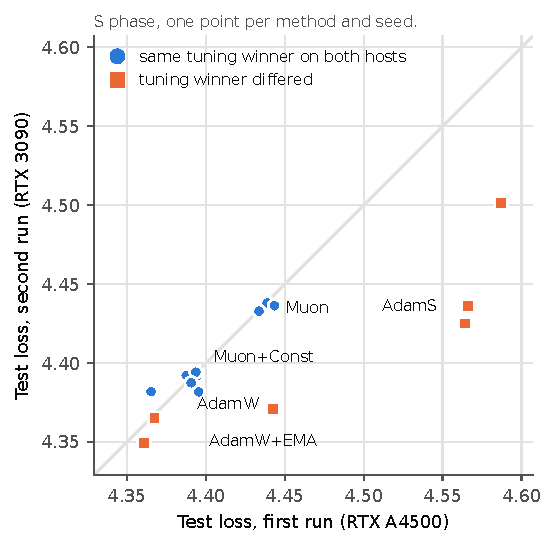
\includegraphics[width=0.55\textwidth]{figures/F6_replicate.pdf}
\caption{S phase, test loss of each final seed on the two hosts. Circles: methods whose tuning winner coincided; squares: methods whose winner differed.}
\label{fig:replicate}
\end{figure}

The protocol tunes on one seed because a second tuning seed doubles the cost of the matrix. The replicate shows the price: for methods near an instability boundary, non-deterministic GPU kernels change which configuration wins, and the edge rule can amplify the change. We report the 3090 run as the main result because it is the complete run that the protocol prescribed; the A4500 run is released with it.

\subsection{More Seeds}
\label{sec:seeds}

Three checks add final seeds to the registered winners. Each starts from the registered run journal of its method, adds seeds, writes its own result file and never replaces a pre-registered one. Appendix~\ref{app:sensitivity} lists every run.

\paragraph{Six seeds at XS.}
Seeds 1004--1006 were added for AdamW and the six methods closest to it in the primary table. AdamW reaches 4.470 (sd 0.033) over six seeds. AdamW+EMA ($-0.013$, CI95 $[-0.043, +0.009]$) and Muon ($-0.006$, $[-0.032, +0.013]$) stay within 0.015 nats of AdamW with intervals that include zero. Muon+Const ($+0.028$), AdamW+dropout ($+0.030$, $[+0.002, +0.053]$) and AdamS ($+0.062$) lose slightly. CWD at its registered winner loses $+0.081$ ($[+0.041, +0.121]$, $p = 0.018$, Holm 0.11). No contrast reaches the Holm criterion. Six seeds narrow the intervals by about half for AdamW+EMA, Muon, Muon+Const and AdamW+dropout, leave those of AdamS and CWD as wide as before, and confirm the three-seed ranking: no method in the top group separates from AdamW.

\paragraph{Six seeds at S.}
Seeds 1004--1006 were added for AdamW and AdamW+EMA at S. AdamW reaches 4.3845 (sd 0.0114) and AdamW+EMA 4.3734 (sd 0.0153). The paired difference is $-0.011$ nats (CI95 $[-0.025, +0.003]$, $p = 0.21$). The three registered seeds gave $-0.027$, $-0.033$ and $-0.011$; the three added seeds give $+0.012$, $+0.011$ and $-0.018$. The registered estimate of $-0.024$ was the favourable half of a small effect. At $n = 6$ the gain is not established, and the equivalence test within 0.01 nats fails as well. The standard deviation of the paired difference for this pair is 0.019 nats at $n = 6$ against 0.011 at $n = 3$.

\paragraph{A third seed in the control arm.}
Seed 1003 was added in arm R1 for all thirteen methods. AdamW reaches 4.183 (sd 0.059). Muon leads by $-0.269$ nats ($[-0.329, -0.214]$). CPR ($-0.068$), CWD ($-0.057$), Baseline ($-0.040$) and Muon+Const ($-0.012$) sit below AdamW. AdamW+EMA ($+0.090$), AdamW+dropout ($+0.116$), the constant decays ($+0.16$ to $+0.27$) and SF-AdamW ($+0.552$) lose. Const-Fair is the only contrast that survives Holm (0.021). The ranking of Section~\ref{sec:r1} is unchanged, except that Muon+Const moves from just above AdamW ($+0.001$) to just below it.

\subsection{A Second Tuning Seed}
\label{sec:tune43}

The registered grids of AdamW, AdamW+EMA and Muon at XS were tuned again on seed 43, without final runs. AdamW and Muon pick the same winner on both seeds (AdamW: lr $4.5\times10^{-3}$, wd 2.5; Muon: lr 0.06, wd 0.1), and in both cases the runner-up trails by more than 0.04 nats. AdamW+EMA does not: seed 42 picks ema 0.99 and seed 43 picks ema 0.9, and on seed 43 the two candidates are 0.012 nats apart. The configurations whose winners are stable are those that the two-host replicate of Section~\ref{sec:replicate} reproduced to 0.003 nats; the unstable one is of the kind that moved there. A second tuning seed therefore detects the fragile winners at the cost of one more grid.

\subsection{Grid Edges}
\label{sec:edges}

The protocol allows one extension per axis. After it, the winners of AdamW, CWD, Muon, Muon+Const and the three constant decays at XS, and of AdamW at S, still sat on the edge of their second axis. We applied a second extension, with the same factor as the first, to every one of them. Five other winners also sat on an edge after the first extension and did not receive a second one: AdamW+dropout (dropout 0.03) and SF-AdamW (wd 2.5) at XS, which later received wd 7.5 in the audit of Section~\ref{sec:sf}, and AdamW+EMA (ema 0.9999), Muon (wd 0.1) and Muon+Const ($\rho = 2.5\times10^{-3}$) at S. Table~\ref{tab:edges} gives the best tuning-seed validation loss on each value of the extended axis.

\begin{table}[t]
\centering
\footnotesize
\begin{tabular}{@{}llllll@{}}
\toprule
Method & axis & registered values & added & winner after & moved \\
\midrule
AdamW (XS) & wd & 0.1, 0.5, 2.5 & 7.5 & 2.5 & no \\
AdamW (S) & wd & 0.1, 0.5, 2.5 & 7.5 & 2.5 & no \\
Muon (XS) & wd & 0.005, 0.02, 0.1 & 0.5 & 0.1 & no \\
Const (XS) & $\rho$ & 1e-4, 5e-4, 2.5e-3 & 1.25e-2 & 2.5e-3 & no \\
Const-Fair (XS) & $\rho$ & 1e-4, 5e-4, 2.5e-3 & 1.25e-2 & 2.5e-3 & no \\
Const-Huber (XS) & $\rho$ & 1e-4, 5e-4, 2.5e-3 & 1.25e-2 & 2.5e-3 & no \\
Muon+Const (XS) & $\rho$ & 1e-4, 5e-4, 2.5e-3 & 1.25e-2 & 2.5e-3 & no \\
CWD (XS) & wd & 0.1, 0.5, 2.5 & 7.5 & 7.5 & yes (Section~\ref{sec:cwd}) \\
\bottomrule
\end{tabular}
\caption{Second extension of the axes on which a registered winner sat after the first extension. ``Winner after'' is the argmin of the tuning-seed validation loss over the extended grid.}
\label{tab:edges}
\end{table}

Seven of the eight winners do not move: the added value loses at every learning rate, so the optimum lies inside the extended grid. For AdamW at XS the step from wd 2.5 to 7.5 raises the best validation loss from 4.485 to 5.077, and for the constant decays the step to $\rho = 1.25\times10^{-2}$ raises it by 0.45 to 0.70 nats. The registered tables therefore compare every method except CWD at its grid optimum. CWD moves to wd 7.5; Section~\ref{sec:cwd} reports it.

\subsection{Schedule-Free AdamW}
\label{sec:sf}

SF-AdamW is the worst method in both regimes. We audited the implementation: the run uses the reference package, receives the warm-up length, uses no external schedule, switches the optimizer between its training and evaluation states around every evaluation, and applies the weight decay after the Adam normalization with the same per-step rate as AdamW. In the repeated-data arm both the training loss and the validation loss of SF-AdamW lag AdamW throughout the run (training loss 4.65 to 4.72 against 3.85 to 3.96 at the last step of the three final runs). With its default weighting, the evaluated iterate is a uniform average of all post-warm-up iterates, and 2,432 steps are too few for that average to catch up. A wider grid confirms that the gap is not under-tuning. We added learning rates $4\times10^{-2}$ and 0.12 and weight decay 7.5 to the registered grid. Every added point loses to the registered winner: at wd 2.5 the validation loss rises from 4.919 to 5.257, 6.026 and 6.763 as the learning rate grows from $4.5\times10^{-3}$ to 0.12, and wd 7.5 adds 0.6 to 0.7 nats at every learning rate.

\section{Post-registration Findings}
\label{sec:post}

The checks of Section~\ref{sec:robustness} ask whether the registered results hold. This section reports what they found beyond the registered matrix, together with four additions decided after the matrix: the control arm at S, one more method, one more model size, and a pre-registered confirmation of the CWD result. None of these results enters the registered tables. One of them, the result on CWD, comes from an extension of the grid; we applied that extension with one rule to the winners listed in Table~\ref{tab:edges}, and only CWD moved.

\subsection{Cautious Weight Decay at Higher Rates}
\label{sec:cwd}

CWD applies the decay only to the coordinates where the update moves the weight toward zero, that is, where the update and the weight have the same sign \citep{chen2026cautious}. Under the registered grid its winner sat at wd 2.5, the edge, and it lost to AdamW by 0.04 nats with three seeds and by 0.08 nats with six. With the second extension, CWD wins at wd 7.5 (Figure~\ref{fig:cwd}). Its final runs reach 4.392 against 4.487 for AdamW on the same three seeds, a difference of $-0.095$ nats (CI95 $[-0.154, -0.061]$, $p = 0.084$). AdamW at the same decay loses 0.6 nats. The cautious mask therefore lets the optimizer use a decay three times stronger than AdamW tolerates, and that stronger decay pays under repetition.

\begin{figure}[t]
\centering
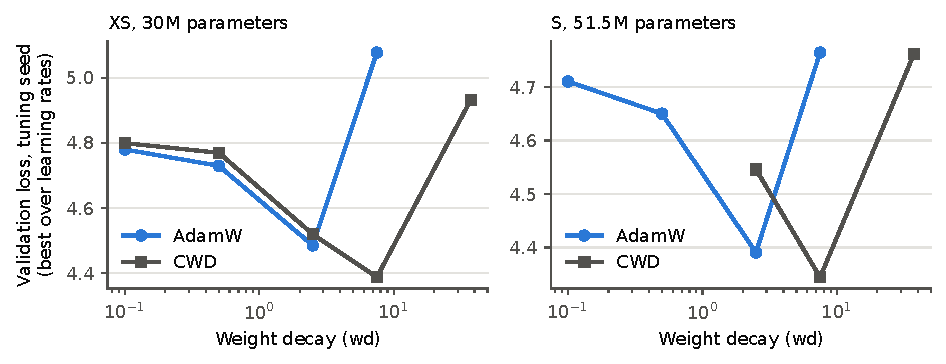
\includegraphics[width=\textwidth]{figures/F7_cwd_wd.pdf}
\caption{Arm R16, tuning seed: best validation loss over the learning-rate grid against the weight decay, for AdamW and CWD. AdamW peaks at wd 2.5 at both sizes; CWD peaks at wd 7.5 and loses at 37.5.}
\label{fig:cwd}
\end{figure}

A further step to wd 37.5 loses at every learning rate at XS (best validation loss 4.932 against 4.387), so wd 7.5 is an interior optimum. At S, CWD searched over lr $\{1.5, 4.5, 13.5\}\times10^{-3}$ and wd $\{2.5, 7.5, 37.5\}$ also picks lr $4.5\times10^{-3}$ and wd 7.5, inside the grid on both axes. Its three final runs reach 4.315 (sd 0.004) against 4.385 for AdamW on the same seeds: a paired difference of $-0.070$ nats, with every seed between $-0.063$ and $-0.081$ (CI95 $[-0.081, -0.063]$, $p = 0.005$). AdamW at wd 7.5 at S loses at every learning rate. The gain of CWD is thus the largest of any method at either size, and it holds at both. Because the result was found after registration, we test it in a separate pre-registered protocol on held-out seeds (Section~\ref{sec:p2}).

\subsection{A Larger Model}
\label{sec:m}

We trained the three leading methods at 124.5M parameters in arm R16, re-tuning the learning rate over three values at the second-axis value tuned at S, with three final seeds. AdamW reaches 4.371 (sd 0.013). AdamW+EMA improves on it by $-0.043$ nats (CI95 $[-0.049, -0.034]$, $p = 0.011$), Muon loses by $+0.063$ ($[+0.050, +0.080]$, $p = 0.019$). Muon's best checkpoint falls at epoch 8, and its final checkpoint is 1.30 nats worse than its best (5.732 against 4.434): the memorization seen at S grows with size. All three winners sit on the largest learning rate of the grid, so these numbers are a size check, not a tuned comparison. For AdamW, protocol P2 later added lr $2.25\times10^{-3}$ and $9\times10^{-3}$ at M and found $4.5\times10^{-3}$ to be an interior optimum (Section~\ref{sec:p2}). Within that limit, the ordering of the three methods at 124.5M is the ordering at S, and the gain of the EMA grows with size ($-0.024$ at XS and S with three seeds, $-0.043$ at 124.5M).

\subsection{The Control Arm at 51.5M Parameters}
\label{sec:r1s}

To check that the regime effect is not a property of the small model, we ran AdamW, AdamW+EMA and Muon in arm R1 at S, each over its R16 winner at S and one weaker variant, with two final seeds. AdamW reaches 4.122. Muon improves on it by $-0.313$ nats (CI95 $[-0.333, -0.293]$), against $+0.051$ in arm R16 at S: a regime effect (R16 contrast minus R1 contrast) of $+0.36$ nats, larger than the $+0.22$ at XS. AdamW+EMA loses by $+0.020$ in R1, against $-0.024$ in R16. At 51.5M parameters, as at 30.4M, Muon's advantage belongs to the single-pass regime and the EMA's small advantage to the repeated one.

\subsection{AdEMAMix}
\label{sec:ademamix}

AdEMAMix \citep{pagliardini2025ademamix} adds a slow momentum to Adam. We first ran it with the settings recommended by its reference implementation (betas 0.9, 0.999, 0.9999; $\alpha = 8$; $\alpha$ and $\beta_3$ warmed up over the whole run) on lr $\{0.5, 1.5, 4.5, 13.5\}\times10^{-3}$ and wd $\{0.1, 0.5, 2.5\}$. At every grid point the norm of the decayed weights grew without bound (from 115 to over 3,600 at the winner, while AdamW's falls from 116 to 91), and the validation loss stalled near 5.9 nats in both arms. We then tuned the slow momentum itself in arm R16 at XS: $\alpha \in \{2, 4\}$, $\beta_3 \in \{0.999, 0.9999\}$, lr $\{0.15, 0.5, 1.5\}\times10^{-3}$, wd 2.5. With $\beta_3 = 0.9999$ the weight norm still grows (up to 2,186) and the best validation loss is 5.42. With $\beta_3 = 0.999$ training is stable (weight norm 116 to 189). The winner, lr $1.5\times10^{-3}$, $\alpha = 2$, $\beta_3 = 0.999$, sits on the edge of all three axes, in the direction of plain Adam: a smaller weight on a shorter slow momentum. Its three final runs reach 4.648 against 4.487 for AdamW on the same seeds, a difference of $+0.161$ nats (per seed $+0.069$ to $+0.226$). At 2,432 steps the slow momentum gives no benefit, and the best configuration moves toward AdamW. AdEMAMix was designed for runs of tens of thousands of steps; we report this result as specific to our horizon.

\subsection{A Pre-registered Confirmation of the CWD Result}
\label{sec:p2}

The CWD result was found by a post-registration extension and selected on the seeds that report it. We therefore fixed a second protocol before running it (protocol P2, committed to the repository with its date). It uses held-out final seeds (2001--2006), gives AdamW the intermediate decays 3.75 and 5 so that a lower effective decay is within its reach, and tests three hypotheses: CWD beats AdamW at S (primary; paired $t$-test at $\alpha = 0.05$ with a bootstrap CI95 below zero), the gain grows with the number of epochs at XS (arms R1, R4 and R16 at identical compute), and the gain holds at 124.5M parameters. Every run logs the fraction of decayed coordinates where the update and the weight agree in sign, from which we report the effective decay of CWD.
Table~\ref{tab:p2} reports the five cells. The edge rule extended the learning-rate grid in three cells: AdamW in R1 and R4 at XS (to $5\times10^{-4}$) and CWD at M (to $1.8\times10^{-2}$); after the extensions no winner sits on a learning-rate edge. No other deviation from the protocol occurred.

\begin{table}[t]
\centering
\footnotesize
\resizebox{\textwidth}{!}{% generated by analysis/p2_analysis.py; do not edit by hand
\begin{tabular}{@{}lllrllrrrccr@{}}
\toprule
Test & Size & Arm & $n$ & CWD winner & AdamW winner & CWD & AdamW & diff & t CI95 & bootstrap CI95 & $p$ \\
\midrule
H1 & S (51.5M) & R16 & 6 & 0.0045, 7.5 & 0.0045, 2.5 & 4.317 & 4.382 & $-0.065$ & $[-0.080, -0.050]$ & $[-0.077, -0.055]$ & 0.0001 \\
H2 & XS (30.4M) & R1 & 3 & 0.0045, 2.5 & 0.0015, 0.5 & 4.110 & 4.128 & $-0.019$ & $[-0.044, +0.006]$ & $[-0.027, -0.008]$ & 0.0857 \\
H2 & XS (30.4M) & R4 & 3 & 0.0045, 2.5 & 0.0015, 0.5 & 4.159 & 4.157 & $+0.002$ & $[-0.009, +0.013]$ & $[-0.001, +0.007]$ & 0.5005 \\
H2 & XS (30.4M) & R16 & 3 & 0.0045, 7.5 & 0.0045, 2.5 & 4.385 & 4.454 & $-0.068$ & $[-0.109, -0.028]$ & $[-0.085, -0.052]$ & 0.0181 \\
H3 & M (124.5M) & R16 & 3 & 0.009, 7.5 & 0.0045, 2.5 & 4.321 & 4.375 & $-0.054$ & $[-0.164, +0.056]$ & $[-0.104, -0.018]$ & 0.1681 \\
\bottomrule
\end{tabular}
}
\caption{Protocol P2: CWD against AdamW on held-out seeds (2001--2006 at S, 2001--2003 at XS and M). Winners are given as lr, wd. Test loss means in nats; diff is the mean paired difference CWD $-$ AdamW with its bootstrap CI95 and the two-sided paired $t$-test.}
\label{tab:p2}
\end{table}

\paragraph{H1 is confirmed.} At S both methods pick the same learning rate as in Section~\ref{sec:cwd}, $4.5\times10^{-3}$. CWD picks wd 7.5, inside its grid; AdamW picks wd 2.5, which is inside its grid once the P1 points at wd 0.1 and 0.5 are counted. On the six held-out seeds CWD reaches 4.317 (sd 0.006) and AdamW 4.382 (sd 0.013). CWD is lower on every seed, by 0.046 to 0.089 nats. The mean paired difference is $-0.065$ nats (bootstrap CI95 $[-0.077, -0.055]$, $t_5 = -11.0$, $p = 0.0001$). It exceeds the practical threshold of 0.03 nats and lies within 0.006 nats of the post-registration estimate on seeds 1001--1003 ($-0.070$).

\paragraph{H2 meets its registered criterion, but the pattern is not monotone.} At XS the paired difference is $-0.019$ nats in R1 (CI95 $[-0.027, -0.008]$), $+0.002$ in R4 ($[-0.001, +0.007]$) and $-0.068$ in R16 ($[-0.085, -0.052]$). The least-squares slope against $\log_2$ of the number of epochs is $-0.012$ nats per doubling, with bootstrap CI95 $[-0.017, -0.008]$, below zero as the protocol requires. The ordinary least-squares $p$-value of the slope is 0.055, and 0.11 after Holm correction. The slope comes from R16: the gain is clear with sixteen epochs and small or absent with one or four. In R1 and R4 the AdamW winner sits on the smallest decay of the grid, wd 0.5, so a lower decay might improve AdamW there. We read H2 as follows: the gain of CWD is a property of heavy repetition, and the data do not show a gradual growth with the number of epochs.

\paragraph{H3: the sign holds at 124.5M parameters.} At M, CWD (lr $9\times10^{-3}$, wd 7.5) reaches 4.321 and AdamW (lr $4.5\times10^{-3}$, wd 2.5) 4.375. CWD is lower on all three seeds, by 0.018 to 0.104 nats. The mean difference is $-0.054$ nats (CI95 $[-0.104, -0.018]$, $p = 0.17$, Holm-adjusted 0.17). With three seeds and this spread the result supports the sign of the gain, not its size. Both winners sit on a decay edge of this small grid.

\paragraph{Mechanism.} Over the final runs, the fraction of decayed coordinates where the update and the weight agree in sign averages 0.40 for CWD at S (0.37 to 0.44 across the five cells). The effective decay of CWD at S, wd times that fraction, is therefore $7.5 \times 0.40 = 3.0$, close to AdamW's tuned 2.5 (1.1 against 0.5 in R1 and R4, 2.8 against 2.5 at M). A lower effective decay does not explain the gain. AdamW's grid brackets CWD's effective value, with wd 2.5 just below it and 3.75 just above, and AdamW stays above CWD at every decay on the tuning seed: 4.391 at wd 2.5, 4.431 at 3.75 and 4.617 at 5, against 4.344 for CWD. The agreement fraction under AdamW is almost the same, 0.41, so the two optimizers apply a similar total shrinkage. They differ in where they apply it. AdamW also shrinks the 60\% of coordinates whose update moves them away from zero; CWD leaves those coordinates alone and applies a stronger decay to the rest.

\section{Discussion}
\label{sec:discussion}

Under sixteen-fold repetition, strong decoupled weight decay is the operating point. The tuned decay rate ($\mathrm{lr} \times \wdec = 0.011$ per step at peak) is one to two orders of magnitude above the values common in single-pass pretraining. \citet{kim2026infinite} report an optimal decay 30 times above standard practice when epoching over fixed data, and \citet{lovelace2026prescriptive} attribute the effect to a lower overfitting coefficient; our tuned value points the same way. The methods that cannot reach such a rate, or that apply it on a different schedule, lose. The three post-step constant decays lose by 0.13 to 0.28 nats in both regimes, and none has a regime effect whose interval excludes zero: the schedule of the decay does not matter once its strength and the learning rate are tuned together, and a constant rate is not a substitute for a rate tied to the learning-rate schedule.

The result on CWD sharpens this reading. AdamW shrinks every coordinate, including those where the update moves the weight away from zero; there the decay works against the gradient signal, and beyond wd 2.5 that conflict costs more than the shrinkage gains. CWD shrinks only the coordinates where the update already moves the weight toward zero. It avoids the conflict and can use a decay three times stronger. Its effective decay, averaged over all decayed coordinates, stays close to AdamW's (3.0 against 2.5 at S), and AdamW does not reach CWD's loss at that decay. The gain therefore comes from where the decay acts, not from how much decay is applied in total. A second pre-registered protocol on held-out seeds confirms the gain at S ($-0.065$ nats). The gain is clear at sixteen epochs, small or absent at one and four, and has the same sign at 124.5M parameters. Under heavy repetition the useful decay is stronger than AdamW can apply without fighting the gradient, and a mask that removes the fight lets the optimizer reach it.

The exponential moving average is the only addition that never loses to AdamW under repetition: $-0.024$ nats at both sizes with three seeds, $-0.011$ nats at S with six, at 0.1\% cost. The six-seed interval, $[-0.025, +0.003]$, includes zero. The effect, if real, is of the order of 0.01 nats, below what three seeds resolve. It is also regime-specific: in the single-pass arm the EMA hurts by 0.13 nats, because the average lags a model that is still improving fast.

Muon illustrates why the control arm matters. Its $-0.24$ nats in the single-pass arm reproduce the gains reported in the literature. Under repetition the gain disappears at XS and reverses at S, and the method memorizes the corpus after ten epochs. A practitioner who repeats data should pair Muon with early stopping or with a stronger decay than its native one; our grid did not find such a configuration within one extension.

The protocol itself produced a result. Two runs of the same phase on two GPUs agreed to 0.003 nats where the tuning winner coincided and differed by up to 0.12 nats where it did not. Single-seed tuning is standard practice in benchmarks of this size. Our replicate quantifies what it costs and suggests two remedies: a second tuning seed for the configurations within one step of the winner, or a report of the tuning-winner variance next to the final-seed variance.

\section{Limitations}
\label{sec:limitations}

The study has three seeds per cell in the main arm and two in the control arm. The standard deviation of the paired difference from AdamW is 0.04 to 0.07 nats at XS (median 0.05; AdamW's own seed-to-seed standard deviation is 0.042) and 0.004 to 0.035 nats at S (median 0.009). A paired $t$-test with three seeds at 80\% power and $\alpha = 0.05$ therefore detects differences of about 0.16 nats at XS and 0.03 nats at S for a typical pair. The six-seed check of Section~\ref{sec:seeds} shows that a three-seed estimate of this standard deviation is itself uncertain: for the EMA contrast at S it rose from 0.011 to 0.019 nats, and six seeds detect 0.027 nats for that pair. The Holm criterion is out of reach at XS, where only the bootstrap intervals carry information, and the XS primary table cannot distinguish methods within 0.1 nats of AdamW from it. The tuning uses one seed, and Section~\ref{sec:replicate} shows what that costs. Five winners still sit on an edge of their second axis (Section~\ref{sec:edges}), so their tuned values are bounds, not optima. The result on CWD comes from an extension beyond the registered grid; a separate pre-registered protocol confirms it at S on six held-out seeds (Section~\ref{sec:p2}), but its tests at XS across regimes and at 124.5M rest on three seeds per cell, and in four of those cells at least one winner sits on a decay edge. At 2,432 steps AdEMAMix trains stably only with a short slow momentum and then loses to AdamW; longer horizons may change that result. The study covers one architecture family, one corpus, sizes from 30M to 125M parameters with the full matrix only at 30M, and one horizon of 2,432 steps. It says nothing about frontier-scale pretraining.

\section{Conclusion}
\label{sec:conclusion}

We compared thirteen regularization methods for language-model pretraining under data repetition with a protocol that tunes every method at equal cost, pairs the final seeds, controls the data regime at identical compute and fixes the analysis in advance. In the registered matrix, tuned AdamW with strong decoupled decay is not beaten. An exponential moving average of the weights gives a gain of 0.01 to 0.02 nats that six seeds do not separate from zero. Constant post-step decays, constrained parameter regularization and schedule-free optimization lose under repetition. Muon's advantage belongs to the single-pass regime. One grid extension found that cautious weight decay, at three times AdamW's decay, beats AdamW under sixteen-fold repetition. A second pre-registered protocol confirms that gain on held-out seeds at 51M parameters, finds it clear only under heavy repetition, and finds the same sign at 124.5M parameters; a lower effective decay does not explain it. An independent replicate shows that single-seed tuning on non-deterministic hardware moves results by up to 0.12 nats, which benchmarks at this scale should report.

\acks{[Funding: to be declared, or ``This work received no external funding.''] The authors declare no competing financial interests. The code, the protocol, the run journals, every result file with its loss curves, the replicate and the analysis script with its tests are available at \url{https://github.com/Metabolic-Intelligence-Lab/Transformer_regularization}. The corpus is pinned by revision and by the SHA-256 of each split.}

\appendix

\section{Tuning Grids}
\label{app:grids}

% generated by analysis/p1_latex_tables.py; do not edit by hand

\subsection*{XS, R16 (10M tokens $\times$ 16 epochs)}

Tuning-seed validation loss at the best checkpoint for every grid point, with the epoch of that checkpoint in parentheses; the winner is the minimum. Rows: learning rate; columns: the second axis.

\footnotesize

\textbf{AdamS} (columns: wd)

\begin{tabular}{@{}lrrr@{}}
\toprule
lr & 1e-05 & 0.0001 & 0.001 \\
\midrule
0.0005 & 4.8510 (16) & 4.8814 (16) & 5.4085 (15) \\
0.0015 & 4.7845 (9) & 4.6918 (11) & 4.9471 (16) \\
0.0045 & 5.0701 (11) & 4.5697 (15) & 5.0050 (16) \\
0.0135 & 6.5184 (16) & 4.5207 (16) & 5.3034 (16) \\
\bottomrule
\end{tabular}

\medskip

\textbf{AdamW} (columns: wd)

\begin{tabular}{@{}lrrr@{}}
\toprule
lr & 0.1 & 0.5 & 2.5 \\
\midrule
0.0005 & 4.8646 (16) & 4.8697 (16) & 5.0901 (16) \\
0.0015 & 4.7794 (10) & 4.7291 (11) & 4.7016 (15) \\
0.0045 & 5.1424 (12) & 4.8492 (14) & 4.4847 (16) \\
0.0135 & 6.4880 (16) & 5.5631 (16) & 4.6892 (16) \\
\bottomrule
\end{tabular}

\medskip

\textbf{AdamW+EMA} (columns: ema)

\begin{tabular}{@{}lrrr@{}}
\toprule
lr & 0.9 & 0.99 & 0.999 \\
\midrule
0.0005 & 5.0668 (14) & 5.0558 (15) & 5.0678 (15.5) \\
0.0015 & 4.6879 (14) & 4.6338 (14) & 4.6253 (15) \\
0.0045 & 4.5023 (16) & 4.4652 (16) & 4.4981 (16) \\
0.0135 & 4.6281 (16) & 4.7495 (16) & 4.8376 (16) \\
\bottomrule
\end{tabular}

\medskip

\textbf{AdamW+dropout} (columns: dropout)

\begin{tabular}{@{}lrrr@{}}
\toprule
lr & 0.03 & 0.1 & 0.3 \\
\midrule
0.0005 & 5.0451 (16) & 5.0533 (16) & 5.2651 (16) \\
0.0015 & 4.6140 (16) & 4.6924 (16) & 4.9022 (16) \\
0.0045 & 4.4603 (16) & 4.5542 (16) & 4.8238 (16) \\
0.0135 & 4.7462 (16) & 4.8383 (16) & 5.0241 (16) \\
\bottomrule
\end{tabular}

\medskip

\textbf{Baseline}

\begin{tabular}{@{}lr@{}}
\toprule
lr & val loss \\
\midrule
0.0005 & 4.8797 (16) \\
0.0015 & 4.8435 (9) \\
0.0045 & 5.2196 (11) \\
\bottomrule
\end{tabular}

\medskip

\textbf{CPR} (columns: warm start)

\begin{tabular}{@{}lrrr@{}}
\toprule
lr & 0 & 250 & 1000 \\
\midrule
0.0005 & 4.8827 (16) & 4.9625 (15) & 4.8736 (16) \\
0.0015 & 4.7901 (10) & 4.7003 (11) & 4.8267 (10) \\
0.0045 & 5.1533 (11) & 4.8663 (13) & 5.1411 (12) \\
\bottomrule
\end{tabular}

\medskip

\textbf{CWD} (columns: wd)

\begin{tabular}{@{}lrrr@{}}
\toprule
lr & 0.1 & 0.5 & 2.5 \\
\midrule
0.0005 & 4.8783 (16) & 4.8582 (16) & 4.8990 (15) \\
0.0015 & 4.7989 (9) & 4.7692 (10) & 4.6678 (11) \\
0.0045 & 5.1900 (11) & 5.0093 (11) & 4.5191 (15) \\
0.0135 & 6.5065 (16) & 6.4191 (16) & 4.8108 (16) \\
\bottomrule
\end{tabular}

\medskip

\textbf{Const} (columns: $\rho$)

\begin{tabular}{@{}lrrr@{}}
\toprule
lr & 0.0001 & 0.0005 & 0.0025 \\
\midrule
0.0005 & 4.8763 (16) & 5.0254 (13) & 5.6858 (8) \\
0.0015 & 4.8021 (10) & 4.7101 (12) & 4.9010 (11) \\
0.0045 & 5.2337 (12) & 4.9521 (16) & 4.6834 (14) \\
0.0135 & 6.5127 (16) & 6.6104 (16) & 5.9457 (15.5) \\
\bottomrule
\end{tabular}

\medskip

\textbf{Const-Fair} (columns: $\rho$)

\begin{tabular}{@{}lrrr@{}}
\toprule
lr & 0.0001 & 0.0005 & 0.0025 \\
\midrule
0.0005 & 4.8697 (16) & 4.9418 (14) & 5.5777 (8) \\
0.0015 & 4.8164 (9) & 4.7196 (11) & 4.7725 (12) \\
0.0045 & 5.1662 (11) & 5.0744 (12) & 4.7121 (15) \\
0.0135 & 6.4810 (16) & 6.5576 (16) & 6.4127 (16) \\
\bottomrule
\end{tabular}

\medskip

\textbf{Const-Huber} (columns: $\rho$)

\begin{tabular}{@{}lrrr@{}}
\toprule
lr & 0.0001 & 0.0005 & 0.0025 \\
\midrule
0.0005 & 4.8493 (16) & 5.0223 (13) & 5.6832 (8) \\
0.0015 & 4.8085 (10) & 4.7261 (11) & 4.8771 (12) \\
0.0045 & 5.1844 (11) & 4.9978 (16) & 4.6348 (14) \\
0.0135 & 6.5287 (16) & 6.5153 (16) & 6.3570 (15.5) \\
\bottomrule
\end{tabular}

\medskip

\textbf{Muon} (columns: wd)

\begin{tabular}{@{}lrrr@{}}
\toprule
lr & 0.005 & 0.02 & 0.1 \\
\midrule
0.007 & 4.7458 (6) & 4.7551 (6) & 4.7211 (6) \\
0.02 & 4.5952 (6) & 4.5875 (6) & 4.5630 (7) \\
0.06 & 4.6182 (9) & 4.5597 (9) & 4.4599 (11) \\
0.18 & 6.6241 (0.5) & 6.6037 (0.5) & 4.5003 (16) \\
\bottomrule
\end{tabular}

\medskip

\textbf{Muon+Const} (columns: $\rho$)

\begin{tabular}{@{}lrrr@{}}
\toprule
lr & 0.0001 & 0.0005 & 0.0025 \\
\midrule
0.007 & 4.7437 (6) & 4.6985 (7) & 4.6767 (9) \\
0.02 & 4.5912 (6) & 4.5535 (7) & 4.5471 (9) \\
0.06 & 4.7325 (16) & 4.5428 (10) & 4.5084 (10) \\
0.18 & 6.6123 (0.5) & 6.6324 (0.5) & 6.4713 (15.5) \\
\bottomrule
\end{tabular}

\medskip

\textbf{SF-AdamW} (columns: wd)

\begin{tabular}{@{}lrrr@{}}
\toprule
lr & 0.1 & 0.5 & 2.5 \\
\midrule
0.0005 & 5.1318 (16) & 5.1347 (16) & 5.2707 (16) \\
0.0015 & 5.0380 (15) & 4.9756 (16) & 5.0355 (16) \\
0.0045 & 5.6090 (16) & 5.2961 (16) & 4.9185 (16) \\
0.0135 & 6.4068 (5.5) & 5.3393 (16) & 5.2565 (16) \\
\bottomrule
\end{tabular}

\medskip

\normalsize

\subsection*{XS, R1 (159.4M tokens $\times$ 1 epoch)}

Tuning-seed validation loss at the best checkpoint for every grid point, with the epoch of that checkpoint in parentheses; the winner is the minimum. Rows: learning rate; columns: the second axis.

\footnotesize

\textbf{AdamS} (columns: wd)

\begin{tabular}{@{}lrr@{}}
\toprule
lr & 2e-05 & 0.0001 \\
\midrule
0.0135 & 6.4826 (1) & 4.2042 (1) \\
\bottomrule
\end{tabular}

\medskip

\textbf{AdamW} (columns: wd)

\begin{tabular}{@{}lrr@{}}
\toprule
lr & 0.5 & 2.5 \\
\midrule
0.0045 & 4.1885 (1) & 4.2773 (1) \\
\bottomrule
\end{tabular}

\medskip

\textbf{AdamW+EMA} (columns: ema)

\begin{tabular}{@{}lrr@{}}
\toprule
lr & 0.9 & 0.99 \\
\midrule
0.0045 & 4.2593 (1) & 4.3042 (1) \\
\bottomrule
\end{tabular}

\medskip

\textbf{AdamW+dropout}

\begin{tabular}{@{}lr@{}}
\toprule
lr & val loss \\
\midrule
0.0045 & 4.3157 (1) \\
\bottomrule
\end{tabular}

\medskip

\textbf{Baseline}

\begin{tabular}{@{}lr@{}}
\toprule
lr & val loss \\
\midrule
0.0015 & 4.1561 (1) \\
\bottomrule
\end{tabular}

\medskip

\textbf{CPR} (columns: warm start)

\begin{tabular}{@{}lrr@{}}
\toprule
lr & 250 & 1000 \\
\midrule
0.0015 & 4.1195 (1) & 4.1531 (1) \\
\bottomrule
\end{tabular}

\medskip

\textbf{CWD} (columns: wd)

\begin{tabular}{@{}lrr@{}}
\toprule
lr & 0.5 & 2.5 \\
\midrule
0.0045 & 4.4240 (1) & 4.1246 (1) \\
\bottomrule
\end{tabular}

\medskip

\textbf{Const} (columns: $\rho$)

\begin{tabular}{@{}lrr@{}}
\toprule
lr & 0.0005 & 0.0025 \\
\midrule
0.0045 & 4.3551 (1) & 4.4806 (0.875) \\
\bottomrule
\end{tabular}

\medskip

\textbf{Const-Fair} (columns: $\rho$)

\begin{tabular}{@{}lrr@{}}
\toprule
lr & 0.0005 & 0.0025 \\
\midrule
0.0045 & 4.4034 (1) & 4.4203 (0.90625) \\
\bottomrule
\end{tabular}

\medskip

\textbf{Const-Huber} (columns: $\rho$)

\begin{tabular}{@{}lrr@{}}
\toprule
lr & 0.0005 & 0.0025 \\
\midrule
0.0045 & 4.3608 (1) & 4.4689 (0.875) \\
\bottomrule
\end{tabular}

\medskip

\textbf{Muon} (columns: wd)

\begin{tabular}{@{}lrr@{}}
\toprule
lr & 0.02 & 0.1 \\
\midrule
0.06 & 3.9771 (1) & 3.9479 (1) \\
\bottomrule
\end{tabular}

\medskip

\textbf{Muon+Const} (columns: $\rho$)

\begin{tabular}{@{}lrr@{}}
\toprule
lr & 0.0005 & 0.0025 \\
\midrule
0.06 & 4.2261 (0.96875) & 4.4112 (0.75) \\
\bottomrule
\end{tabular}

\medskip

\textbf{SF-AdamW} (columns: wd)

\begin{tabular}{@{}lrr@{}}
\toprule
lr & 0.5 & 2.5 \\
\midrule
0.0045 & 4.8769 (1) & 4.6753 (1) \\
\bottomrule
\end{tabular}

\medskip

\normalsize

\subsection*{S, R16 (10M tokens $\times$ 16 epochs)}

Tuning-seed validation loss at the best checkpoint for every grid point, with the epoch of that checkpoint in parentheses; the winner is the minimum. Rows: learning rate; columns: the second axis.

\footnotesize

\textbf{AdamS} (columns: wd)

\begin{tabular}{@{}lrrr@{}}
\toprule
lr & 1e-05 & 0.0001 & 0.001 \\
\midrule
0.0005 & 4.7780 (11) & 4.7563 (12) & 5.2742 (15) \\
0.0015 & 4.7172 (8) & 4.5563 (10) & 4.7736 (16) \\
0.0045 & 6.2235 (4) & 4.5506 (15) & 5.0157 (16) \\
0.0135 & 6.7059 (16) & 4.4359 (16) & 5.3021 (16) \\
\bottomrule
\end{tabular}

\medskip

\textbf{AdamW} (columns: wd)

\begin{tabular}{@{}lrrr@{}}
\toprule
lr & 0.1 & 0.5 & 2.5 \\
\midrule
0.0005 & 4.7773 (11) & 4.7688 (12) & 4.8726 (14) \\
0.0015 & 4.7106 (8) & 4.6504 (9) & 4.5207 (14) \\
0.0045 & 6.3233 (3) & 4.9047 (15) & 4.3905 (16) \\
0.0135 & 6.6861 (16) & 6.3398 (16) & 4.6823 (16) \\
\bottomrule
\end{tabular}

\medskip

\textbf{AdamW+EMA} (columns: ema)

\begin{tabular}{@{}lrrr@{}}
\toprule
lr & 0.99 & 0.999 & 0.9999 \\
\midrule
0.0005 & 4.8695 (13) & 4.8590 (14) & 4.8501 (14) \\
0.0015 & 4.4436 (13) & 4.4315 (14) & 4.4371 (13) \\
0.0045 & 4.4201 (15.5) & 4.4051 (16) & 4.3893 (16) \\
0.0135 & 4.7017 (16) & 4.8058 (16) & 4.7965 (16) \\
\bottomrule
\end{tabular}

\medskip

\textbf{Muon} (columns: wd)

\begin{tabular}{@{}lrrr@{}}
\toprule
lr & 0.005 & 0.02 & 0.1 \\
\midrule
0.007 & 4.7494 (5) & 4.7201 (5) & 4.6857 (5) \\
0.02 & 4.6061 (5) & 4.5825 (6) & 4.5314 (6) \\
0.06 & 5.5637 (2.5) & 4.5937 (11) & 4.4523 (10) \\
0.18 & 6.5715 (0.5) & 6.5683 (0.5) & 4.4913 (16) \\
\bottomrule
\end{tabular}

\medskip

\textbf{Muon+Const} (columns: $\rho$)

\begin{tabular}{@{}lrrr@{}}
\toprule
lr & 0.0001 & 0.0005 & 0.0025 \\
\midrule
0.007 & 4.7355 (5) & 4.6750 (5) & 4.5647 (8) \\
0.02 & 4.5997 (5) & 4.5438 (6) & 4.4411 (9) \\
0.06 & 5.6500 (2) & 5.4646 (15.5) & 4.4108 (11) \\
0.18 & 6.5728 (0.5) & 6.5793 (0.5) & 6.2993 (15.5) \\
\bottomrule
\end{tabular}

\medskip

\normalsize



\section{Sensitivity Tables}
\label{app:sensitivity}

% generated by analysis/p1_latex_tables.py; do not edit by hand

\subsection*{XS, R16 (D = 10M $\times$ 16 epochs) --- tag \texttt{add}: method outside the protocol (AdEMAMix), tuned on the extended AdamW grid}

\footnotesize
\resizebox{\textwidth}{!}{%
\begin{tabular}{@{}lllrlll@{}}
\toprule
Method & winner & tuning val & $n$ & test loss & registered winner & registered test \\
\midrule
AdEMAMix & lr 0.0005, wd 0.1 & 5.9134 & 3 & 5.8874 $\pm$ 0.0098 & -- & -- \\
\bottomrule
\end{tabular}}
\normalsize

\footnotesize
\noindent
\textbf{AdEMAMix} (columns: wd)

\begin{tabular}{@{}lrrr@{}}
\toprule
lr & 0.1 & 0.5 & 2.5 \\
\midrule
0.0005 & 5.9134 (4) & 5.9424 (3.5) & 5.9247 (3.5) \\
0.0015 & 5.9470 (4) & 5.9857 (5.5) & 5.9957 (3.5) \\
0.0045 & 6.5673 (3.5) & 6.5066 (3) & 6.2577 (16) \\
0.0135 & 6.9446 (1.5) & 6.9447 (1.5) & 6.3855 (16) \\
\bottomrule
\end{tabular}

\medskip

\normalsize

\subsection*{XS, R1 (D = 159.4M $\times$ 1 epoch) --- tag \texttt{add}: method outside the protocol (AdEMAMix), tuned on the extended AdamW grid}

\footnotesize
\resizebox{\textwidth}{!}{%
\begin{tabular}{@{}lllrlll@{}}
\toprule
Method & winner & tuning val & $n$ & test loss & registered winner & registered test \\
\midrule
AdEMAMix & lr 0.0005, wd 0.1 & 5.8452 & 2 & 5.8065 $\pm$ 0.0034 & -- & -- \\
\bottomrule
\end{tabular}}
\normalsize

\footnotesize
\noindent
\textbf{AdEMAMix} (columns: wd)

\begin{tabular}{@{}lrr@{}}
\toprule
lr & 0.02 & 0.1 \\
\midrule
0.0005 & 5.8679 (0.3125) & 5.8452 (0.28125) \\
\bottomrule
\end{tabular}

\medskip

\normalsize

\subsection*{XS, R16 (D = 10M $\times$ 16 epochs) --- tag \texttt{add2}: AdEMAMix with alpha and beta3 tuned (reference values diverge at this horizon), wd 2.5}

\footnotesize
\resizebox{\textwidth}{!}{%
\begin{tabular}{@{}lllrlll@{}}
\toprule
Method & winner & tuning val & $n$ & test loss & registered winner & registered test \\
\midrule
AdEMAMix-T & lr 0.0015, alpha 2, beta3 0.999, wd 2.5 & 4.7241 & 3 & 4.6480 $\pm$ 0.0407 & -- & -- \\
\bottomrule
\end{tabular}}
\normalsize

\footnotesize
\noindent
\textbf{AdEMAMix-T} (columns: $\alpha$, $\beta_3$)

\begin{tabular}{@{}lrrrr@{}}
\toprule
lr & 2, 0.999 & 2, 0.9999 & 4, 0.999 & 4, 0.9999 \\
\midrule
0.00015 & 5.1886 (16) & 5.7665 (16) & 5.0149 (16) & 6.0505 (6.5) \\
0.0005 & 4.8968 (11) & 5.4454 (7) & 4.8586 (11) & 5.7688 (4.5) \\
0.0015 & 4.7241 (11) & 5.4241 (16) & 4.7584 (9) & 5.8231 (5) \\
\bottomrule
\end{tabular}

\medskip

\normalsize

\subsection*{XS, R16 (D = 10M $\times$ 16 epochs) --- tag \texttt{audit}: tuning points beyond the protocol grid (no finals)}

\footnotesize
\resizebox{\textwidth}{!}{%
\begin{tabular}{@{}lllrlll@{}}
\toprule
Method & winner & tuning val & $n$ & test loss & registered winner & registered test \\
\midrule
SF-AdamW & lr 0.0045, wd 2.5 & 4.9185 & 0 & -- & same & 4.8992 ($n$=3) \\
\bottomrule
\end{tabular}}
\normalsize

\footnotesize
\noindent
\textbf{SF-AdamW} (columns: wd)

\begin{tabular}{@{}lrr@{}}
\toprule
lr & 2.5 & 7.5 \\
\midrule
0.0045 & 4.9185 (16) & 5.6216 (16) \\
0.0135 & 5.2565 (16) & 5.8884 (16) \\
0.04 & 6.0262 (16) & 6.6446 (11) \\
0.12 & 6.7629 (14.5) & 7.3885 (5) \\
\bottomrule
\end{tabular}

\medskip

\normalsize

\subsection*{S, R16 (D = 10M $\times$ 16 epochs) --- tag \texttt{cwd}: CWD follow-up after its edge winner (wd 7.5): grid closed with wd 37.5 at XS, search at S}

\footnotesize
\resizebox{\textwidth}{!}{%
\begin{tabular}{@{}lllrlll@{}}
\toprule
Method & winner & tuning val & $n$ & test loss & registered winner & registered test \\
\midrule
CWD & lr 0.0045, wd 7.5 & 4.3442 & 3 & 4.3146 $\pm$ 0.0038 & -- & -- \\
\bottomrule
\end{tabular}}
\normalsize

Contrasts against the pre-registered AdamW ($n = 3$):

\footnotesize
\begin{tabular}{@{}lrrrcrr@{}}
\toprule
Method & mean & sd & diff & bootstrap CI95 & $p$ & $p$ (Holm) \\
\midrule
CWD & 4.3146 & 0.0038 & $-0.0705$ & $[-0.0805, -0.0628]$ & 0.005 & 0.005 \\
\bottomrule
\end{tabular}
\normalsize

\footnotesize
\noindent
\textbf{CWD} (columns: wd)

\begin{tabular}{@{}lrrr@{}}
\toprule
lr & 2.5 & 7.5 & 37.5 \\
\midrule
0.0015 & 4.5462 (11) & 4.4515 (14) & 4.7625 (16) \\
0.0045 & 4.5609 (14) & 4.3442 (16) & 4.9459 (16) \\
0.0135 & 4.9454 (16) & 4.4019 (16) & 5.1448 (16) \\
\bottomrule
\end{tabular}

\medskip

\normalsize

\subsection*{XS, R16 (D = 10M $\times$ 16 epochs) --- tag \texttt{cwd}: CWD follow-up after its edge winner (wd 7.5): grid closed with wd 37.5 at XS, search at S}

\footnotesize
\resizebox{\textwidth}{!}{%
\begin{tabular}{@{}lllrlll@{}}
\toprule
Method & winner & tuning val & $n$ & test loss & registered winner & registered test \\
\midrule
CWD & lr 0.0045, wd 7.5 & 4.3869 & 3 & 4.3919 $\pm$ 0.0090 & lr 0.0045, wd 2.5 & 4.5283 ($n$=3) \\
\bottomrule
\end{tabular}}
\normalsize

Contrasts against the pre-registered AdamW ($n = 3$):

\footnotesize
\begin{tabular}{@{}lrrrcrr@{}}
\toprule
Method & mean & sd & diff & bootstrap CI95 & $p$ & $p$ (Holm) \\
\midrule
CWD & 4.3919 & 0.0090 & $-0.0953$ & $[-0.1539, -0.0612]$ & 0.084 & 0.084 \\
\bottomrule
\end{tabular}
\normalsize

\footnotesize
\noindent
\textbf{CWD} (columns: wd)

\begin{tabular}{@{}lrrrrr@{}}
\toprule
lr & 0.1 & 0.5 & 2.5 & 7.5 & 37.5 \\
\midrule
0.0005 & 4.8783 (16) & 4.8582 (16) & 4.8990 (15) & 5.0625 (15) & 5.4016 (14) \\
0.0015 & 4.7989 (9) & 4.7692 (10) & 4.6678 (11) & 4.5749 (14) & 4.9321 (16) \\
0.0045 & 5.1900 (11) & 5.0093 (11) & 4.5191 (15) & 4.3869 (16) & 5.0032 (16) \\
0.0135 & 6.5065 (16) & 6.4191 (16) & 4.8108 (16) & 4.6225 (16) & 5.1336 (16) \\
\bottomrule
\end{tabular}

\medskip

\normalsize

\subsection*{XS, R16 (D = 10M $\times$ 16 epochs) --- tag \texttt{edge}: second extension on the axis where the registered winner still sits on the edge}

\footnotesize
\resizebox{\textwidth}{!}{%
\begin{tabular}{@{}lllrlll@{}}
\toprule
Method & winner & tuning val & $n$ & test loss & registered winner & registered test \\
\midrule
AdamW & lr 0.0045, wd 2.5 & 4.4847 & 3 & 4.4872 $\pm$ 0.0420 & same & 4.4872 ($n$=3) \\
CWD & lr 0.0045, wd 7.5 & 4.3869 & 3 & 4.3919 $\pm$ 0.0090 & lr 0.0045, wd 2.5 & 4.5283 ($n$=3) \\
Const & lr 0.0045, rho 0.0025 & 4.6834 & 3 & 4.6582 $\pm$ 0.0290 & same & 4.6582 ($n$=3) \\
Const-Fair & lr 0.0045, rho 0.0025, delta 0.1 & 4.7121 & 3 & 4.7539 $\pm$ 0.0810 & same & 4.7539 ($n$=3) \\
Const-Huber & lr 0.0045, rho 0.0025, delta 0.1 & 4.6348 & 3 & 4.6192 $\pm$ 0.0411 & same & 4.6192 ($n$=3) \\
Muon & lr 0.06, wd 0.1, aux\_lr 0.0015, aux\_wd 0.1 & 4.4599 & 3 & 4.4661 $\pm$ 0.0051 & same & 4.4661 ($n$=3) \\
Muon+Const & lr 0.06, rho 0.0025, aux\_lr 0.0015 & 4.5084 & 3 & 4.4978 $\pm$ 0.0057 & same & 4.4978 ($n$=3) \\
\bottomrule
\end{tabular}}
\normalsize

The AdamW winner is the registered one; its finals on seeds 1001, 1002, 1003 are the registered runs.

Contrasts against the tagged AdamW ($n = 3$):

\footnotesize
\begin{tabular}{@{}lrrrcrr@{}}
\toprule
Method & mean & sd & diff & bootstrap CI95 & $p$ & $p$ (Holm) \\
\midrule
CWD & 4.3919 & 0.0090 & $-0.0953$ & $[-0.1539, -0.0612]$ & 0.084 & 0.333 \\
Muon & 4.4661 & 0.0051 & $-0.0212$ & $[-0.0670, +0.0024]$ & 0.454 & 0.908 \\
Muon+Const & 4.4978 & 0.0057 & $+0.0105$ & $[-0.0429, +0.0450]$ & 0.735 & 0.908 \\
Const-Huber & 4.6192 & 0.0411 & $+0.1320$ & $[+0.0672, +0.2070]$ & 0.083 & 0.333 \\
Const & 4.6582 & 0.0290 & $+0.1709$ & $[+0.1269, +0.2258]$ & 0.028 & 0.139 \\
Const-Fair & 4.7539 & 0.0810 & $+0.2667$ & $[+0.2057, +0.3069]$ & 0.013 & 0.080 \\
\bottomrule
\end{tabular}
\normalsize

\footnotesize
\noindent
\textbf{AdamW} (columns: wd)

\begin{tabular}{@{}lrrrr@{}}
\toprule
lr & 0.1 & 0.5 & 2.5 & 7.5 \\
\midrule
0.0005 & 4.8646 (16) & 4.8697 (16) & 5.0901 (16) & 5.4991 (16) \\
0.0015 & 4.7794 (10) & 4.7291 (11) & 4.7016 (15) & 5.0769 (16) \\
0.0045 & 5.1424 (12) & 4.8492 (14) & 4.4847 (16) & 5.0821 (16) \\
0.0135 & 6.4880 (16) & 5.5631 (16) & 4.6892 (16) & 5.3739 (16) \\
\bottomrule
\end{tabular}

\medskip

\textbf{CWD} (columns: wd)

\begin{tabular}{@{}lrrrr@{}}
\toprule
lr & 0.1 & 0.5 & 2.5 & 7.5 \\
\midrule
0.0005 & 4.8783 (16) & 4.8582 (16) & 4.8990 (15) & 5.0625 (15) \\
0.0015 & 4.7989 (9) & 4.7692 (10) & 4.6678 (11) & 4.5749 (14) \\
0.0045 & 5.1900 (11) & 5.0093 (11) & 4.5191 (15) & 4.3869 (16) \\
0.0135 & 6.5065 (16) & 6.4191 (16) & 4.8108 (16) & 4.6225 (16) \\
\bottomrule
\end{tabular}

\medskip

\textbf{Const} (columns: $\rho$)

\begin{tabular}{@{}lrrrr@{}}
\toprule
lr & 0.0001 & 0.0005 & 0.0025 & 0.0125 \\
\midrule
0.0005 & 4.8763 (16) & 5.0254 (13) & 5.6858 (8) & 6.5046 (5) \\
0.0015 & 4.8021 (10) & 4.7101 (12) & 4.9010 (11) & 5.8857 (7) \\
0.0045 & 5.2337 (12) & 4.9521 (16) & 4.6834 (14) & 5.5621 (10) \\
0.0135 & 6.5127 (16) & 6.6104 (16) & 5.9457 (15.5) & 5.3850 (12.5) \\
\bottomrule
\end{tabular}

\medskip

\textbf{Const-Fair} (columns: $\rho$)

\begin{tabular}{@{}lrrrr@{}}
\toprule
lr & 0.0001 & 0.0005 & 0.0025 & 0.0125 \\
\midrule
0.0005 & 4.8697 (16) & 4.9418 (14) & 5.5777 (8) & 6.4619 (5) \\
0.0015 & 4.8164 (9) & 4.7196 (11) & 4.7725 (12) & 5.7873 (8) \\
0.0045 & 5.1662 (11) & 5.0744 (12) & 4.7121 (15) & 5.3499 (11.5) \\
0.0135 & 6.4810 (16) & 6.5576 (16) & 6.4127 (16) & 5.5053 (13.5) \\
\bottomrule
\end{tabular}

\medskip

\textbf{Const-Huber} (columns: $\rho$)

\begin{tabular}{@{}lrrrr@{}}
\toprule
lr & 0.0001 & 0.0005 & 0.0025 & 0.0125 \\
\midrule
0.0005 & 4.8493 (16) & 5.0223 (13) & 5.6832 (8) & 6.5009 (5) \\
0.0015 & 4.8085 (10) & 4.7261 (11) & 4.8771 (12) & 5.8883 (8.5) \\
0.0045 & 5.1844 (11) & 4.9978 (16) & 4.6348 (14) & 5.5908 (11.5) \\
0.0135 & 6.5287 (16) & 6.5153 (16) & 6.3570 (15.5) & 5.0873 (13) \\
\bottomrule
\end{tabular}

\medskip

\textbf{Muon} (columns: wd)

\begin{tabular}{@{}lrrrr@{}}
\toprule
lr & 0.005 & 0.02 & 0.1 & 0.5 \\
\midrule
0.007 & 4.7458 (6) & 4.7551 (6) & 4.7211 (6) & 4.7169 (9) \\
0.02 & 4.5952 (6) & 4.5875 (6) & 4.5630 (7) & 4.6075 (14) \\
0.06 & 4.6182 (9) & 4.5597 (9) & 4.4599 (11) & 4.6415 (16) \\
0.18 & 6.6241 (0.5) & 6.6037 (0.5) & 4.5003 (16) & 4.6369 (16) \\
\bottomrule
\end{tabular}

\medskip

\textbf{Muon+Const} (columns: $\rho$)

\begin{tabular}{@{}lrrrr@{}}
\toprule
lr & 0.0001 & 0.0005 & 0.0025 & 0.0125 \\
\midrule
0.007 & 4.7437 (6) & 4.6985 (7) & 4.6767 (9) & 5.7454 (7) \\
0.02 & 4.5912 (6) & 4.5535 (7) & 4.5471 (9) & 5.4187 (7) \\
0.06 & 4.7325 (16) & 4.5428 (10) & 4.5084 (10) & 5.2340 (7.5) \\
0.18 & 6.6123 (0.5) & 6.6324 (0.5) & 6.4713 (15.5) & 5.6321 (11.5) \\
\bottomrule
\end{tabular}

\medskip

\normalsize

\subsection*{M (124.5M parameters), R16 (D = 10M $\times$ 16 epochs) --- tag \texttt{m}: spot check at 124.5M parameters: S-tuned second axis, learning rate re-tuned, three finals}

\footnotesize
\resizebox{\textwidth}{!}{%
\begin{tabular}{@{}lllrlll@{}}
\toprule
Method & winner & tuning val & $n$ & test loss & registered winner & registered test \\
\midrule
AdamW & lr 0.0045, wd 2.5 & 4.3853 & 3 & 4.3711 $\pm$ 0.0134 & -- & -- \\
AdamW+EMA & lr 0.0045, ema 0.9999, wd 2.5 & 4.3086 & 3 & 4.3277 $\pm$ 0.0066 & -- & -- \\
Muon & lr 0.06, wd 0.1, aux\_lr 0.0015, aux\_wd 0.1 & 4.4518 & 3 & 4.4339 $\pm$ 0.0023 & -- & -- \\
\bottomrule
\end{tabular}}
\normalsize

Contrasts against the tagged AdamW ($n = 3$):

\footnotesize
\begin{tabular}{@{}lrrrcrr@{}}
\toprule
Method & mean & sd & diff & bootstrap CI95 & $p$ & $p$ (Holm) \\
\midrule
AdamW+EMA & 4.3277 & 0.0066 & $-0.0434$ & $[-0.0493, -0.0344]$ & 0.011 & 0.022 \\
Muon & 4.4339 & 0.0023 & $+0.0628$ & $[+0.0502, +0.0798]$ & 0.019 & 0.022 \\
\bottomrule
\end{tabular}
\normalsize

\footnotesize
\noindent
\textbf{AdamW}

\begin{tabular}{@{}lr@{}}
\toprule
lr & val loss \\
\midrule
0.0005 & 4.6405 (11) \\
0.0015 & 4.4791 (14) \\
0.0045 & 4.3853 (16) \\
\bottomrule
\end{tabular}

\medskip

\textbf{AdamW+EMA}

\begin{tabular}{@{}lr@{}}
\toprule
lr & val loss \\
\midrule
0.0005 & 4.6172 (12) \\
0.0015 & 4.3630 (13) \\
0.0045 & 4.3086 (15.5) \\
\bottomrule
\end{tabular}

\medskip

\textbf{Muon}

\begin{tabular}{@{}lr@{}}
\toprule
lr & val loss \\
\midrule
0.007 & 4.7226 (4) \\
0.02 & 4.5642 (5) \\
0.06 & 4.4518 (9) \\
\bottomrule
\end{tabular}

\medskip

\normalsize

\subsection*{S, R1 (D = 159.4M $\times$ 1 epoch) --- tag \texttt{r1s}: control arm at S: the R16 winner at S and its weaker variant, two finals}

\footnotesize
\resizebox{\textwidth}{!}{%
\begin{tabular}{@{}lllrlll@{}}
\toprule
Method & winner & tuning val & $n$ & test loss & registered winner & registered test \\
\midrule
AdamW & lr 0.0045, wd 2.5 & 4.1512 & 2 & 4.1221 $\pm$ 0.0063 & -- & -- \\
AdamW+EMA & lr 0.0045, ema 0.99, wd 2.5 & 4.1673 & 2 & 4.1422 $\pm$ 0.0268 & -- & -- \\
Muon & lr 0.06, wd 0.1, aux\_lr 0.0015, aux\_wd 0.1 & 3.7981 & 2 & 3.8091 $\pm$ 0.0225 & -- & -- \\
\bottomrule
\end{tabular}}
\normalsize

Contrasts against the tagged AdamW ($n = 2$):

\footnotesize
\begin{tabular}{@{}lrrrcrr@{}}
\toprule
Method & mean & sd & diff & bootstrap CI95 & $p$ & $p$ (Holm) \\
\midrule
Muon & 3.8091 & 0.0225 & $-0.3130$ & $[-0.3334, -0.2927]$ & 0.041 & 0.083 \\
AdamW+EMA & 4.1422 & 0.0268 & $+0.0200$ & $[+0.0056, +0.0345]$ & 0.398 & 0.398 \\
\bottomrule
\end{tabular}
\normalsize

\footnotesize
\noindent
\textbf{AdamW} (columns: wd)

\begin{tabular}{@{}lrr@{}}
\toprule
lr & 0.5 & 2.5 \\
\midrule
0.0045 & 4.2720 (1) & 4.1512 (1) \\
\bottomrule
\end{tabular}

\medskip

\textbf{AdamW+EMA} (columns: ema)

\begin{tabular}{@{}lrr@{}}
\toprule
lr & 0.99 & 0.9999 \\
\midrule
0.0045 & 4.1673 (1) & 4.2081 (1) \\
\bottomrule
\end{tabular}

\medskip

\textbf{Muon} (columns: wd)

\begin{tabular}{@{}lrr@{}}
\toprule
lr & 0.02 & 0.1 \\
\midrule
0.06 & 4.1437 (1) & 3.7981 (1) \\
\bottomrule
\end{tabular}

\medskip

\normalsize

\subsection*{XS, R16 (D = 10M $\times$ 16 epochs) --- tag \texttt{tune43}: the registered grid tuned again on seed 43 (no finals): variance of the tuning winner}

\footnotesize
\resizebox{\textwidth}{!}{%
\begin{tabular}{@{}lllrlll@{}}
\toprule
Method & winner & tuning val & $n$ & test loss & registered winner & registered test \\
\midrule
AdamW & lr 0.0045, wd 2.5 & 4.4609 & 0 & -- & same & 4.4872 ($n$=3) \\
AdamW+EMA & lr 0.0045, ema 0.9, wd 2.5 & 4.4561 & 0 & -- & lr 0.0045, ema 0.99, wd 2.5 & 4.4637 ($n$=3) \\
Muon & lr 0.06, wd 0.1, aux\_lr 0.0015, aux\_wd 0.1 & 4.4666 & 0 & -- & same & 4.4661 ($n$=3) \\
\bottomrule
\end{tabular}}
\normalsize

\footnotesize
\noindent
\textbf{AdamW} (columns: wd)

\begin{tabular}{@{}lrrr@{}}
\toprule
lr & 0.1 & 0.5 & 2.5 \\
\midrule
0.0005 & 4.8667 (16) & 4.8704 (16) & 5.0361 (16) \\
0.0015 & 4.7768 (9) & 4.7184 (11) & 4.6606 (14) \\
0.0045 & 5.1545 (11) & 4.7931 (14) & 4.4609 (16) \\
0.0135 & 6.5233 (16) & 5.4917 (16) & 4.7849 (16) \\
\bottomrule
\end{tabular}

\medskip

\textbf{AdamW+EMA} (columns: ema)

\begin{tabular}{@{}lrrr@{}}
\toprule
lr & 0.9 & 0.99 & 0.999 \\
\midrule
0.0005 & 5.0577 (15) & 5.0340 (15) & 5.0577 (16) \\
0.0015 & 4.6188 (14) & 4.6187 (13) & 4.6476 (15) \\
0.0045 & 4.4561 (16) & 4.4678 (16) & 4.4971 (16) \\
0.0135 & 4.7631 (16) & 4.6242 (16) & 4.8839 (16) \\
\bottomrule
\end{tabular}

\medskip

\textbf{Muon} (columns: wd)

\begin{tabular}{@{}lrrr@{}}
\toprule
lr & 0.005 & 0.02 & 0.1 \\
\midrule
0.007 & 4.7503 (6) & 4.7463 (6) & 4.7260 (6) \\
0.02 & 4.6099 (6) & 4.6051 (6) & 4.5754 (7) \\
0.06 & 4.6068 (9) & 4.5234 (9) & 4.4666 (11) \\
0.18 & 6.6124 (0.5) & 6.6213 (0.5) & 4.5108 (16) \\
\bottomrule
\end{tabular}

\medskip

\normalsize

\subsection*{S, R16 (D = 10M $\times$ 16 epochs) --- tag \texttt{wdx}: second weight-decay extension of the AdamW grid (wd 7.5), beyond the one the protocol allows}

\footnotesize
\resizebox{\textwidth}{!}{%
\begin{tabular}{@{}lllrlll@{}}
\toprule
Method & winner & tuning val & $n$ & test loss & registered winner & registered test \\
\midrule
AdamW & lr 0.0045, wd 2.5 & 4.3905 & 3 & 4.3851 $\pm$ 0.0059 & same & 4.3851 ($n$=3) \\
\bottomrule
\end{tabular}}
\normalsize

The AdamW winner is the registered one; its finals on seeds 1001, 1002, 1003 are the registered runs.

\footnotesize
\noindent
\textbf{AdamW} (columns: wd)

\begin{tabular}{@{}lrrrr@{}}
\toprule
lr & 0.1 & 0.5 & 2.5 & 7.5 \\
\midrule
0.0005 & 4.7773 (11) & 4.7688 (12) & 4.8726 (14) & 5.2737 (15) \\
0.0015 & 4.7106 (8) & 4.6504 (9) & 4.5207 (14) & 4.7647 (16) \\
0.0045 & 6.3233 (3) & 4.9047 (15) & 4.3905 (16) & 4.9345 (16) \\
\bottomrule
\end{tabular}

\medskip

\normalsize

\subsection*{XS, R1 (D = 159.4M $\times$ 1 epoch) --- tag \texttt{x3}: a third final seed (1003) in the control arm}

\footnotesize
\resizebox{\textwidth}{!}{%
\begin{tabular}{@{}lllrlll@{}}
\toprule
Method & winner & tuning val & $n$ & test loss & registered winner & registered test \\
\midrule
AdamS & lr 0.0135, wd 0.0001 & 4.2042 & 3 & 4.2228 $\pm$ 0.0281 & same & 4.2294 ($n$=2) \\
AdamW & lr 0.0045, wd 0.5 & 4.1885 & 3 & 4.1827 $\pm$ 0.0587 & same & 4.1529 ($n$=2) \\
AdamW+EMA & lr 0.0045, ema 0.9, wd 2.5 & 4.2593 & 3 & 4.2725 $\pm$ 0.0125 & same & 4.2793 ($n$=2) \\
AdamW+dropout & lr 0.0045, dropout 0.03, wd 2.5 & 4.3157 & 3 & 4.2987 $\pm$ 0.0122 & same & 4.3043 ($n$=2) \\
Baseline & lr 0.0015 & 4.1561 & 3 & 4.1428 $\pm$ 0.0024 & same & 4.1414 ($n$=2) \\
CPR & lr 0.0015, warm\_start 250 & 4.1195 & 3 & 4.1152 $\pm$ 0.0073 & same & 4.1155 ($n$=2) \\
CWD & lr 0.0045, wd 2.5 & 4.1246 & 3 & 4.1258 $\pm$ 0.0047 & same & 4.1285 ($n$=2) \\
Const & lr 0.0045, rho 0.0005 & 4.3551 & 3 & 4.3468 $\pm$ 0.0340 & same & 4.3316 ($n$=2) \\
Const-Fair & lr 0.0045, rho 0.0005, delta 0.1 & 4.4034 & 3 & 4.4519 $\pm$ 0.0475 & same & 4.4328 ($n$=2) \\
Const-Huber & lr 0.0045, rho 0.0005, delta 0.1 & 4.3608 & 3 & 4.4075 $\pm$ 0.0682 & same & 4.4076 ($n$=2) \\
Muon & lr 0.06, wd 0.1, aux\_lr 0.0015, aux\_wd 0.1 & 3.9479 & 3 & 3.9142 $\pm$ 0.0036 & same & 3.9148 ($n$=2) \\
Muon+Const & lr 0.06, rho 0.0005, aux\_lr 0.0015 & 4.2261 & 3 & 4.1706 $\pm$ 0.0488 & same & 4.1535 ($n$=2) \\
SF-AdamW & lr 0.0045, wd 2.5 & 4.6753 & 3 & 4.7345 $\pm$ 0.0163 & same & 4.7430 ($n$=2) \\
\bottomrule
\end{tabular}}
\normalsize

The AdamW winner is the registered one; its finals on seeds 1001, 1002 are the registered runs.

Contrasts against the tagged AdamW ($n = 3$):

\footnotesize
\begin{tabular}{@{}lrrrcrr@{}}
\toprule
Method & mean & sd & diff & bootstrap CI95 & $p$ & $p$ (Holm) \\
\midrule
Muon & 3.9142 & 0.0036 & $-0.2685$ & $[-0.3294, -0.2136]$ & 0.015 & 0.137 \\
CPR & 4.1152 & 0.0073 & $-0.0675$ & $[-0.1279, -0.0167]$ & 0.173 & 0.891 \\
CWD & 4.1258 & 0.0047 & $-0.0569$ & $[-0.1220, +0.0032]$ & 0.257 & 1.000 \\
Baseline & 4.1428 & 0.0024 & $-0.0399$ & $[-0.0968, +0.0165]$ & 0.347 & 1.000 \\
Muon+Const & 4.1706 & 0.0488 & $-0.0121$ & $[-0.0660, +0.0673]$ & 0.794 & 1.000 \\
AdamS & 4.2228 & 0.0281 & $+0.0401$ & $[-0.0328, +0.0787]$ & 0.386 & 1.000 \\
AdamW+EMA & 4.2725 & 0.0125 & $+0.0898$ & $[+0.0165, +0.1501]$ & 0.149 & 0.891 \\
AdamW+dropout & 4.2987 & 0.0122 & $+0.1160$ & $[+0.0451, +0.1868]$ & 0.105 & 0.736 \\
Const & 4.3468 & 0.0340 & $+0.1641$ & $[+0.1349, +0.1852]$ & 0.008 & 0.083 \\
Const-Huber & 4.4075 & 0.0682 & $+0.2248$ & $[+0.1586, +0.3509]$ & 0.070 & 0.564 \\
Const-Fair & 4.4519 & 0.0475 & $+0.2692$ & $[+0.2478, +0.2860]$ & 0.002 & 0.021 \\
SF-AdamW & 4.7345 & 0.0163 & $+0.5518$ & $[+0.4753, +0.6110]$ & 0.005 & 0.058 \\
\bottomrule
\end{tabular}
\normalsize

\footnotesize
\noindent
\textbf{AdamS} (columns: wd)

\begin{tabular}{@{}lrr@{}}
\toprule
lr & 2e-05 & 0.0001 \\
\midrule
0.0135 & 6.4826 (1) & 4.2042 (1) \\
\bottomrule
\end{tabular}

\medskip

\textbf{AdamW} (columns: wd)

\begin{tabular}{@{}lrr@{}}
\toprule
lr & 0.5 & 2.5 \\
\midrule
0.0045 & 4.1885 (1) & 4.2773 (1) \\
\bottomrule
\end{tabular}

\medskip

\textbf{AdamW+EMA} (columns: ema)

\begin{tabular}{@{}lrr@{}}
\toprule
lr & 0.9 & 0.99 \\
\midrule
0.0045 & 4.2593 (1) & 4.3042 (1) \\
\bottomrule
\end{tabular}

\medskip

\textbf{AdamW+dropout}

\begin{tabular}{@{}lr@{}}
\toprule
lr & val loss \\
\midrule
0.0045 & 4.3157 (1) \\
\bottomrule
\end{tabular}

\medskip

\textbf{Baseline}

\begin{tabular}{@{}lr@{}}
\toprule
lr & val loss \\
\midrule
0.0015 & 4.1561 (1) \\
\bottomrule
\end{tabular}

\medskip

\textbf{CPR} (columns: warm start)

\begin{tabular}{@{}lrr@{}}
\toprule
lr & 250 & 1000 \\
\midrule
0.0015 & 4.1195 (1) & 4.1531 (1) \\
\bottomrule
\end{tabular}

\medskip

\textbf{CWD} (columns: wd)

\begin{tabular}{@{}lrr@{}}
\toprule
lr & 0.5 & 2.5 \\
\midrule
0.0045 & 4.4240 (1) & 4.1246 (1) \\
\bottomrule
\end{tabular}

\medskip

\textbf{Const} (columns: $\rho$)

\begin{tabular}{@{}lrr@{}}
\toprule
lr & 0.0005 & 0.0025 \\
\midrule
0.0045 & 4.3551 (1) & 4.4806 (0.875) \\
\bottomrule
\end{tabular}

\medskip

\textbf{Const-Fair} (columns: $\rho$)

\begin{tabular}{@{}lrr@{}}
\toprule
lr & 0.0005 & 0.0025 \\
\midrule
0.0045 & 4.4034 (1) & 4.4203 (0.90625) \\
\bottomrule
\end{tabular}

\medskip

\textbf{Const-Huber} (columns: $\rho$)

\begin{tabular}{@{}lrr@{}}
\toprule
lr & 0.0005 & 0.0025 \\
\midrule
0.0045 & 4.3608 (1) & 4.4689 (0.875) \\
\bottomrule
\end{tabular}

\medskip

\textbf{Muon} (columns: wd)

\begin{tabular}{@{}lrr@{}}
\toprule
lr & 0.02 & 0.1 \\
\midrule
0.06 & 3.9771 (1) & 3.9479 (1) \\
\bottomrule
\end{tabular}

\medskip

\textbf{Muon+Const} (columns: $\rho$)

\begin{tabular}{@{}lrr@{}}
\toprule
lr & 0.0005 & 0.0025 \\
\midrule
0.06 & 4.2261 (0.96875) & 4.4112 (0.75) \\
\bottomrule
\end{tabular}

\medskip

\textbf{SF-AdamW} (columns: wd)

\begin{tabular}{@{}lrr@{}}
\toprule
lr & 0.5 & 2.5 \\
\midrule
0.0045 & 4.8769 (1) & 4.6753 (1) \\
\bottomrule
\end{tabular}

\medskip

\normalsize

\subsection*{S, R16 (D = 10M $\times$ 16 epochs) --- tag \texttt{x6}: six final seeds (1004-1006 added) under the pre-registered winners}

\footnotesize
\resizebox{\textwidth}{!}{%
\begin{tabular}{@{}lllrlll@{}}
\toprule
Method & winner & tuning val & $n$ & test loss & registered winner & registered test \\
\midrule
AdamW & lr 0.0045, wd 2.5 & 4.3905 & 6 & 4.3845 $\pm$ 0.0114 & same & 4.3851 ($n$=3) \\
AdamW+EMA & lr 0.0045, ema 0.9999, wd 2.5 & 4.3893 & 6 & 4.3734 $\pm$ 0.0153 & same & 4.3615 ($n$=3) \\
\bottomrule
\end{tabular}}
\normalsize

The AdamW winner is the registered one; its finals on seeds 1001, 1002, 1003 are the registered runs.

Contrasts against the tagged AdamW ($n = 6$):

\footnotesize
\begin{tabular}{@{}lrrrcrr@{}}
\toprule
Method & mean & sd & diff & bootstrap CI95 & $p$ & $p$ (Holm) \\
\midrule
AdamW+EMA & 4.3734 & 0.0153 & $-0.0111$ & $[-0.0245, +0.0027]$ & 0.206 & 0.206 \\
\bottomrule
\end{tabular}
\normalsize

\footnotesize
\noindent
\textbf{AdamW} (columns: wd)

\begin{tabular}{@{}lrrr@{}}
\toprule
lr & 0.1 & 0.5 & 2.5 \\
\midrule
0.0005 & 4.7773 (11) & 4.7688 (12) & 4.8726 (14) \\
0.0015 & 4.7106 (8) & 4.6504 (9) & 4.5207 (14) \\
0.0045 & 6.3233 (3) & 4.9047 (15) & 4.3905 (16) \\
\bottomrule
\end{tabular}

\medskip

\textbf{AdamW+EMA} (columns: ema)

\begin{tabular}{@{}lrrr@{}}
\toprule
lr & 0.99 & 0.999 & 0.9999 \\
\midrule
0.0005 & 4.8695 (13) & 4.8590 (14) & 4.8501 (14) \\
0.0015 & 4.4436 (13) & 4.4315 (14) & 4.4371 (13) \\
0.0045 & 4.4201 (15.5) & 4.4051 (16) & 4.3893 (16) \\
\bottomrule
\end{tabular}

\medskip

\normalsize

\subsection*{XS, R16 (D = 10M $\times$ 16 epochs) --- tag \texttt{x6}: six final seeds (1004-1006 added) under the pre-registered winners}

\footnotesize
\resizebox{\textwidth}{!}{%
\begin{tabular}{@{}lllrlll@{}}
\toprule
Method & winner & tuning val & $n$ & test loss & registered winner & registered test \\
\midrule
AdamS & lr 0.0135, wd 0.0001 & 4.5207 & 6 & 4.5310 $\pm$ 0.0687 & same & 4.4914 ($n$=3) \\
AdamW & lr 0.0045, wd 2.5 & 4.4847 & 6 & 4.4695 $\pm$ 0.0331 & same & 4.4872 ($n$=3) \\
AdamW+EMA & lr 0.0045, ema 0.99, wd 2.5 & 4.4652 & 6 & 4.4570 $\pm$ 0.0149 & same & 4.4637 ($n$=3) \\
AdamW+dropout & lr 0.0045, dropout 0.03, wd 2.5 & 4.4603 & 6 & 4.4992 $\pm$ 0.0186 & same & 4.5005 ($n$=3) \\
CWD & lr 0.0045, wd 2.5 & 4.5191 & 6 & 4.5507 $\pm$ 0.0335 & same & 4.5283 ($n$=3) \\
Muon & lr 0.06, wd 0.1, aux\_lr 0.0015, aux\_wd 0.1 & 4.4599 & 6 & 4.4641 $\pm$ 0.0054 & same & 4.4661 ($n$=3) \\
Muon+Const & lr 0.06, rho 0.0025, aux\_lr 0.0015 & 4.5084 & 6 & 4.4970 $\pm$ 0.0040 & same & 4.4978 ($n$=3) \\
\bottomrule
\end{tabular}}
\normalsize

The AdamW winner is the registered one; its finals on seeds 1001, 1002, 1003 are the registered runs.

Contrasts against the tagged AdamW ($n = 6$):

\footnotesize
\begin{tabular}{@{}lrrrcrr@{}}
\toprule
Method & mean & sd & diff & bootstrap CI95 & $p$ & $p$ (Holm) \\
\midrule
AdamW+EMA & 4.4570 & 0.0149 & $-0.0126$ & $[-0.0434, +0.0085]$ & 0.439 & 0.879 \\
Muon & 4.4641 & 0.0054 & $-0.0055$ & $[-0.0322, +0.0131]$ & 0.686 & 0.879 \\
Muon+Const & 4.4970 & 0.0040 & $+0.0275$ & $[-0.0022, +0.0461]$ & 0.115 & 0.480 \\
AdamW+dropout & 4.4992 & 0.0186 & $+0.0296$ & $[+0.0015, +0.0534]$ & 0.096 & 0.480 \\
AdamS & 4.5310 & 0.0687 & $+0.0615$ & $[-0.0032, +0.1275]$ & 0.157 & 0.480 \\
CWD & 4.5507 & 0.0335 & $+0.0811$ & $[+0.0405, +0.1208]$ & 0.018 & 0.106 \\
\bottomrule
\end{tabular}
\normalsize

\footnotesize
\noindent
\textbf{AdamS} (columns: wd)

\begin{tabular}{@{}lrrr@{}}
\toprule
lr & 1e-05 & 0.0001 & 0.001 \\
\midrule
0.0005 & 4.8510 (16) & 4.8814 (16) & 5.4085 (15) \\
0.0015 & 4.7845 (9) & 4.6918 (11) & 4.9471 (16) \\
0.0045 & 5.0701 (11) & 4.5697 (15) & 5.0050 (16) \\
0.0135 & 6.5184 (16) & 4.5207 (16) & 5.3034 (16) \\
\bottomrule
\end{tabular}

\medskip

\textbf{AdamW} (columns: wd)

\begin{tabular}{@{}lrrr@{}}
\toprule
lr & 0.1 & 0.5 & 2.5 \\
\midrule
0.0005 & 4.8646 (16) & 4.8697 (16) & 5.0901 (16) \\
0.0015 & 4.7794 (10) & 4.7291 (11) & 4.7016 (15) \\
0.0045 & 5.1424 (12) & 4.8492 (14) & 4.4847 (16) \\
0.0135 & 6.4880 (16) & 5.5631 (16) & 4.6892 (16) \\
\bottomrule
\end{tabular}

\medskip

\textbf{AdamW+EMA} (columns: ema)

\begin{tabular}{@{}lrrr@{}}
\toprule
lr & 0.9 & 0.99 & 0.999 \\
\midrule
0.0005 & 5.0668 (14) & 5.0558 (15) & 5.0678 (15.5) \\
0.0015 & 4.6879 (14) & 4.6338 (14) & 4.6253 (15) \\
0.0045 & 4.5023 (16) & 4.4652 (16) & 4.4981 (16) \\
0.0135 & 4.6281 (16) & 4.7495 (16) & 4.8376 (16) \\
\bottomrule
\end{tabular}

\medskip

\textbf{AdamW+dropout} (columns: dropout)

\begin{tabular}{@{}lrrr@{}}
\toprule
lr & 0.03 & 0.1 & 0.3 \\
\midrule
0.0005 & 5.0451 (16) & 5.0533 (16) & 5.2651 (16) \\
0.0015 & 4.6140 (16) & 4.6924 (16) & 4.9022 (16) \\
0.0045 & 4.4603 (16) & 4.5542 (16) & 4.8238 (16) \\
0.0135 & 4.7462 (16) & 4.8383 (16) & 5.0241 (16) \\
\bottomrule
\end{tabular}

\medskip

\textbf{CWD} (columns: wd)

\begin{tabular}{@{}lrrr@{}}
\toprule
lr & 0.1 & 0.5 & 2.5 \\
\midrule
0.0005 & 4.8783 (16) & 4.8582 (16) & 4.8990 (15) \\
0.0015 & 4.7989 (9) & 4.7692 (10) & 4.6678 (11) \\
0.0045 & 5.1900 (11) & 5.0093 (11) & 4.5191 (15) \\
0.0135 & 6.5065 (16) & 6.4191 (16) & 4.8108 (16) \\
\bottomrule
\end{tabular}

\medskip

\textbf{Muon} (columns: wd)

\begin{tabular}{@{}lrrr@{}}
\toprule
lr & 0.005 & 0.02 & 0.1 \\
\midrule
0.007 & 4.7458 (6) & 4.7551 (6) & 4.7211 (6) \\
0.02 & 4.5952 (6) & 4.5875 (6) & 4.5630 (7) \\
0.06 & 4.6182 (9) & 4.5597 (9) & 4.4599 (11) \\
0.18 & 6.6241 (0.5) & 6.6037 (0.5) & 4.5003 (16) \\
\bottomrule
\end{tabular}

\medskip

\textbf{Muon+Const} (columns: $\rho$)

\begin{tabular}{@{}lrrr@{}}
\toprule
lr & 0.0001 & 0.0005 & 0.0025 \\
\midrule
0.007 & 4.7437 (6) & 4.6985 (7) & 4.6767 (9) \\
0.02 & 4.5912 (6) & 4.5535 (7) & 4.5471 (9) \\
0.06 & 4.7325 (16) & 4.5428 (10) & 4.5084 (10) \\
0.18 & 6.6123 (0.5) & 6.6324 (0.5) & 6.4713 (15.5) \\
\bottomrule
\end{tabular}

\medskip

\normalsize



\vskip 0.2in
\bibliography{refs}

\end{document}
